\documentclass[a4paper, 12pt]{article} % Font size (can be 10pt, 11pt or 12pt) and paper size (remove a4paper for US letter paper)

\usepackage{graphicx} % Required for including pictures
\usepackage{apacite}
\usepackage{sectsty}
\usepackage{breakcites}
\usepackage[margin=1in]{geometry}
\usepackage[T1]{fontenc}
\usepackage{newtxmath,newtxtext}
 \usepackage{enumitem}
   \usepackage{listings}
    \lstset{
   	basicstyle=\ttfamily,
   	mathescape
   }
 \usepackage{xcolor}

  \newcommand\mycomment[1]{\textcolor{red}{\textbf{\textit{(#1)}}}}
 \newcommand\mycommentn[1]{\textcolor{red}{\textbf{\textit{#1}}}\newline}
 

\makeatletter

\renewcommand{\maketitle}{ % Customize the title - do not edit title and author name here, see the TITLE block below
\begin{flushleft} 
{\large\@title\footnotemark[1]} % Increase the font size of the title

\vspace{20pt} % Some vertical space between the title and author name

{\large\@author} % Author name
\end{flushleft}
}


\sectionfont{\fontsize{12}{15}\selectfont\bfseries}
\subsectionfont{\fontsize{12}{15}\selectfont\bfseries\itshape}

%----------------------------------------------------------------------------------------
%	TITLE
%----------------------------------------------------------------------------------------

\title{\textbf{Stochastic Decision Optimization based on Deterministic Approximations of Processes described as Closed-form Arithmetic Simulation }} % Title
\author{Mohan Krishnamoorthy$^{a,2}$, Alexander Brodsky$^a$, and Daniel A. Menasc\'e$^{a}$} % Author

%----------------------------------------------------------------------------------------

\begin{document}
\pagestyle{empty}
\maketitle % Print the title section

\begin{flushleft} 
\vspace{10pt}
$^a$\textit{Department of Computer Science, George Mason University, Fairfax, Virginia 22030, USA.
% Telephone No.: (703) 993-1537
}\\
\vspace{20pt}
$^a$\{mkrishn4, brodsky, menasce\}@gmu.edu \\
\vspace{20pt}
\textbf{Acknowledgement}\newline
This work was partially supported by NIST Grant No. 70NANB12H277. \newline
\vspace{20pt}
%% To
%{\tiny Provide short biographical notes on all contributors here if the journal requires them\newline Word count: 5691}
\footnotetext[1]{Word Count: 6319 \mycomment{to update}}
\footnotetext[2]{Corresponding Author}
\end{flushleft} 

\newpage
\pagestyle{plain}
\setcounter{page}{1}
\noindent{\large \@title }
\vspace{10pt}
%----------------------------------------------------------------------------------------
%	ABSTRACT AND KEYWORDS
%----------------------------------------------------------------------------------------


\begin{abstract}{\small\noindent
We consider processes with metrics of interest, including process cost, that are stochasticfeasibility constraints and metrics of interest that includes a cost function where the metrics are stochastic functions of the process controls. We propose an efficient stochastic optimization algorithm for the problem of finding process controls that minimize the expectation of cost while satisfying multiple deterministic and stochastic feasibility constraints with a given high probability. The proposed algorithm is based on (1) a series of deterministic approximations to produce a candidate set of near-optimal control settings for the production process, and (2) stochastic simulations on the candidate set using optimal simulation budget allocation methods. In an experimental study, we demonstrate the proposed algorithm on a use case of a real-world heat-sink service network that involves contract suppliers and manufacturers as well as unit manufacturing processes of shearing, milling, drilling, and machining. The experimental study shows that the proposed algorithm significantly outperforms four popular simulation-based stochastic optimization algorithms.
}
\end{abstract}

{\small  Keywords: decision support;
	decision guidance;
	deterministic approximations;
	stochastic simulation optimization;
	heuristic algorithm } % Keywords

\vspace{5pt} % Some vertical space between the abstract and first section

\section{Introduction}

%Motivation
This paper considers a process with feasibility constraints and metrics of interest that includes a cost function where the metrics are stochastic functions of the process controls.
This paper is concerned with the development of a one-stage stochastic optimization algorithm for the problem of finding process controls that minimize the expectation of cost while satisfying multiple deterministic and stochastic feasibility constraints with a given high probability.
These problems are prevalent in manufacturing processes, such as assembly lines and supply chain management where the goal is to find the process controls that minimize the expected cost subject to satisfying deterministic control bound constraints and stochastic steady state demand for the multiple output products with a given high probability. 
There is an increasing need for process analysis and optimization to solve this problem efficiently as companies want to be competitive and need to reduce their cost and improve efficiency of operations in the face of increased global competition. 


%Research Gap
%Current state of the art and its limitations (funnel)
%%high level 
%Simulation based approaches
Stochastic optimization have typically been performed using simulation-based optimization techniques (see \cite{Amaran2016} and \cite{Nguyen2014} for a review of such techniques). 
Tools like SIMULINK \cite{Dabney:2001:MS:557989} and Modelica \cite{elmqvist1998modelica,Provan2012modelica} allow users to run stochastic simulations on models of complex systems in mechanical, hydraulic, thermal, control, and electrical power.
Tools like OMOptim \cite{OMOptim}, Efficient Traceable Model-Based Dynamic Optimization (EDOp) \cite{EDOp}, and jMetal \cite{jMetal} use simulation models to heuristically-guide a trial and error search for the optimal answer. 
However, the general limitation of simulation-based approaches is that simulation is used as a black box, and the underlying mathematical structure is not utilized. 


%NP

From the work on Mathematical Programming (MP), we know that, for deterministic problems, utilizing the mathematical structure can lead to significantly better results in terms of optimality of results and computational complexity compared to simulation-based approaches (see e.g., \cite{Amaran2016} and \cite{Klemmt2009}). 
For this reason, a number of approaches have been developed to bridge the gap between stochastic simulation and MP.
%key things that they do
For instance, \cite{thompson_integrated_1990} propose an integrated approach that combines simulation with MP where the MP problem is constructed from the original stochastic problem with uncertainties being resolved to their mean values by using a sample of black-box simulations. This strategy of extracting an MP from the original problem is also used by \cite{paraskevopoulos_robust_1991} to solve the optimal capacity planning problem by incorporating the original objective function augmented with a penalty on the sensitivity of the objective function to various types of uncertainty.
The authors of \cite{Xu2014MultiFid} propose an ordinal transformation framework, 
consisting of a two-stage optimization framework that first extracts a low fidelity model using simulation or a queuing network model using assumptions that simplify the original problem and then uses this model to reduce the search space over which high fidelity simulations are run to find the optimal solution to the original problem.
%This low fidelity model is in a closed mathematical form and solving this model reduces the search space. High fidelity simulations  are then used on this smaller search space to find the optimal solutions to the original problem.
Other stochastic optimization approaches in the literature try to extract the mathematical structure of the original problem using similar techniques.
However, extraction of the mathematical structure through sampling using a black-box simulation is computationally expensive, especially for real-world processes composed of complex process networks.

%NP
Instead of extracting the mathematical structure using black-box simulation, in \cite{Krishnamoorthy2015}, we used the extraction of mathematical structure from a white-box simulation code analysis as part of a heuristic algorithm to solve a stochastic optimization problem of finding controls for temporal production processes with inventories as to minimize the total cost while satisfying the stochastic demand with a predefined probability.
Similar to the  previous approaches, the mathematical structure was used for approximating a candidate set of solutions by solving a series of deterministic MP problems that approximate the stochastic simulation. 
However, the class of problems considered in \cite{Krishnamoorthy2015} is limited to processes described using piece-wise linear arithmetic. 
Whereas, many processes have models based on physics-based equations with non-linear arithmetic. 

To close this gap, we extended the heuristic algorithm from \cite{Krishnamoorthy2015} to an algorithm called Stochastic Optimization Algorithm based on Deterministic Approximations (SODA) to solve the stochastic optimization problem over a composite service network that involve processes described using non-linear arithmetic \cite{GMU-CS-TR-2017-3}.
However, SODA was limited to production processes with stochastic metrics of cost and throughput and the only stochastic constraint considered in the optimization problem was that of demand satisfaction with sufficient probability. Whereas, many processes have multiple stochastic metrics and the stochastic optimization problem needs to consider the satisfaction of multiple constraints over these stochastic metrics with sufficient probability. 
Hence, in this paper, we generalize SODA to close the gap for stochastic optimization of processes that have feasibility constraints over multiple stochastic metrics while being described using non-linear arithmetic.

%Key contibutions
More specifically, the contributions of this paper are two-fold:
First, we propose a heuristic algorithm called general Stochastic Optimization Algorithm based on Deterministic Approximations (g-SODA) to solve the problem of finding process controls that minimize the expectation of cost while satisfying multiple deterministic and stochastic feasibility constraints with a given high probability. 
The proposed algorithm is based on (1) a series of deterministic approximations to produce a candidate set of near-optimal control settings for the production process, and (2) stochastic simulations on the candidate set using optimal simulation budget allocation methods (e.g., see \cite{Chen2011}, \cite{Lee2012OCBACO}).  
%Second, we demonstrate the proposed algorithm on a use case of a real-world heat-sink production process that involves contract suppliers and manufacturers as well as unit manufacturing processes of shearing, milling, drilling, and machining with models from the literature that use non-linear physics-based equations.
Second, we conduct an initial experimental study over a real world use case of heat-sink service network to compare the proposed algorithm with four popular simulation-based stochastic optimization algorithms viz., Nondominated Sorting Genetic Algorithm 2 (NGSA2) \cite{ngsa2}, Indicator Based Evolutionary Algorithm (IBEA) \cite{ibea}, Strength Pareto Evolutionary Algorithm 2 (SPEA2) \cite{spea2}, and Speed-constrained Multi-objective Particle swarm optimization (SMPSO) \cite{NDG09}.
 The experimental study demonstrates that g-SODA significantly outperforms the other algorithms in terms of optimality of results and computation time. In particular, 
running over a 12-process problem with 22 decision variables and 21 stochastic constraints using a 8-core server with 16GB RAM,
in one day, g-SODA achieves a production cost lower than that of competing algorithms by 42\%; and in three days, g-SODA achieves 25\% better cost.

%Organization
The rest of this paper is organized as follows. Section \ref{sec:prob} formally describes the stochastic optimization problem over processes with multiple stochastic feasibility constraints. The algorithm for g-SODA, including deterministic approximations, is presented in section \ref{sec:algo}. Section \ref{sec:expResults} describes the experimental study to evaluate g-SODA's performance. Finally, section \ref{sec:conclusion} concludes with some future research directions. 


\section{Stochastic Optimization over Processes with Multiple Stochastic Feasibility Constraints and Closed-form Non-linear Arithmetic}
\label{sec:prob}

We now borrow the stochastic optimization problem from \cite{GMU-CS-TR-2017-3} and extend it for  processes that have feasibility constraints over multiple stochastic metrics and are described using non-linear arithmetic.
The stochastic optimization problem for such processes assumes a stochastic closed-form arithmetic (SCFA) simulation of the following form.
A SCFA simulation on input variable $\vec{X}$ is a sequence $y_1=expr_1,\dots,y_n=expr_n$
\newline where $expr_i, 1\le i \le n$ is either
\begin{enumerate}[label=(\alph*)]
	\item An arithmetic or boolean expression in terms of a subset of the elements of $\vec{X}$ and/or $y_1,\dots,y_{i-1}$. We say that $y_i$ is arithmetic or boolean if the $expr_i$ is arithmetic or boolean correspondingly.
	\item An expression invoking $PD(\vec{P})$, which is a function that draws from a probability distribution (e.g., gaussian, exponential, uniform) using parameters $\vec{P}$ that are a subset of the elements of $\vec{X}$ and/or $y_1,\dots,y_{i-1}$.
\end{enumerate}
%y_i is deterministic or stochastic
We say that $y_i, 1\le i \le n$ is stochastic if, recursively,
\begin{enumerate}[label=(\alph*)]
	\item $expr_i$ invokes $PD(\vec{P})$, or
	\item $expr_i$ uses at least one stochastic variable $y_j, 1\le j < i$
\end{enumerate}
If $y_i$ is not stochastic, we say that it is deterministic.
%SCFAI computes variable v if v is y_i for i in 1,...,n
Also, we say that a SCFA simulation $\mathbb{S}$  computes a variable \textit{v} if $v=y_i$, for some $1\le i \le n$.

\noindent To clarify, consider a simple SCFA simulation example that consists of the following sequence of expressions: 
\begin{lstlisting}
1: stochSpeed := speed + $\mathcal{N}$(0,$\sigma$)
2: stochTime := $f$(stochSpeed)
3: throughput := 1/stochTime
4: cost := throughput $\times$ pricePerUnit
5: C := lb $\le$ speed $\le$ ub
\end{lstlisting}
In this example, the SCFA simulation computes the stochastic arithmetic variables of \textit{cost} and \textit{throughput} as well as the deterministic boolean variable \textit{C}.
The variable \textit{speed} is deterministic (e.g., machine speed) and it should be bounded within some lower bound (\textit{lb}) and upper bound (\textit{ub}).
The boolean variable \textit{C} describes whether \textit{speed} is bounded.
Also, the effects of \textit{speed} is stochastic (\textit{stochSpeed}) due to normally distributed random noise $\mathcal{N}(0,\sigma)$. 
For the sake of brevity, say that the stochastic time to produce one item (\textit{stochTime}) is obtained from a function described in terms of \textit{stochSpeed}.
Then, \textit{throughput} is computed as the inverse of \textit{stochTime} and \textit{cost} is computed as the product of \textit{throughput} and a fixed parameter of price to produce one unit of item (\textit{pricePerUnit}).

%Our problem (with C, cost, thru)
This paper considers the stochastic optimization problem of finding process controls that minimize the cost expectation while satisfying multiple deterministic and stochastic feasibility constraints with a given probability.
More formally, the stochastic optimization problem is of the form:
\begin{equation}
\label{eq:stochProb}
\begin{aligned}
& \underset{\vec{X}\in\vec{D}}{\text{minimize}}
& & E(\textit{cost}(\vec{X})) \\
& \text{subject to}
& & C(\vec{X}) \wedge \\
&&& \forall_{i\in\{1,\dots,k\}}P(m_i(\vec{X}) \ge \theta_i) \ge \alpha_i
\end{aligned}
\end{equation}
where $\vec{D} = D_1 \times \dots \times D_n$ is the domain for decision variables $\vec{X}$\\
\indent\indent\indent$\vec{X}$ is a vector of decision variables that range over $\vec{D}$\\
\indent\indent\indent\textit{cost}$(\vec{X})$ is a random variable defined in terms of $\vec{X}$\\
\indent\indent\indent$C(\vec{X})$ is a deterministic constraint in $\vec{X}$ i.e., a function $C:\vec{D} \rightarrow \{true,false\}$\\
%\indent\indent\indent$\mathcal{M}$  is a set of random variables, all defined in terms of $\vec{X}$ and $m_k(\vec{X}) \in \mathcal{M}$\\
\indent\indent\indent $m_1(\vec{X}),\dots,m_k(\vec{X})$ are random variable defined in terms of $\vec{X}$\\
\indent\indent\indent$\theta_1,\dots,\theta_k \in \mathbb{R}^k$ are the constraint thresholds \\
\indent\indent\indent$\alpha_1,\dots,\alpha_k \in [0,1]^k$ are the probability threshold, and\\
\indent\indent\indent$P(m_i(\vec{X}) \ge \theta_i)$ is the probability that $m_i(\vec{X})$ is greater than or equal to $\theta_i$, and\\\indent\indent\indent\indent\indent\indent\indent~$i\in\{1,\dots,k\}$

Note in this problem that upon increasing $\theta_i$ to some $\theta_i'$ where $i\in\{1,\dots,k\}$, the size of the space of alternatives that satisfy the respective stochastic constraint in equation \ref{eq:stochProb} increases and hence it can be said that the best solution, i.e., the minimum expected cost is monotonically improving in $\theta_i'$.

We assume that the random variables, \textit{cost($\vec{X}$)}, $m_1(\vec{X}),\dots,m_k(\vec{X})$ as well as the deterministic constraint $C(\vec{X})$ are expressed by an SCFA simulation $\mathbb{S}$ that computes the corresponding stochastic arithmetic variables \textit{cost}, $m_1,\dots,m_k$ as well as the deterministic boolean variable $C \in \{true, false\}$. 

%While we exemplified the SCFA simulation using a very simple example in this section, many complex real-world processes can be formulated as SCFA simulation such as the use case described in section \ref{sec:expProbSetup}.

%While the SCFA simulation applies to complex real-wold production processes as shown in the use case described in section \ref{sec:expProbSetup}, to make the problem formulation clear, the SCFA simulation of a simple process is presented as an example here.


%
%
%
%\subsection{Convergence of Solutions Involving Monte Carlo Simulation-based Optimization}
%\label{ssec:convergenceProp}
%In order to solve the the stochastic optimization problem described in equation \ref{eq:stochProb}, this paper proposes a simulation based optimization approach with deterministic approximation and heuristics. This approach incorporates the deterministic approximation procedure described in section \ref{ssec:detApproxModel} and then adds noise to the variables of the models to run simulation procedure based on Monte Carlo simulation described in section \ref{ssec:simProc}. In this section, we will show that when the mean of the noise distribution is 0, the noise becomes negligible when the number of simulations is very large due to which it is possible for simulation based optimization approaches to eventually converge to the optimal point. 
%
%If \textit{cost} is the total cost of production as obtained from the deterministic abstraction of the original stochastic problem, then, for \textit{n} sampled values of $\overrightarrow{\mathcal{N}}$, $E(\widehat{cost})_n$ is the expected value of the sample cost. Say that $E(\widehat{cost})$ is its true (population) expected value and suppose that it exist. Since all n sampled values of $\overrightarrow{\mathcal{N}}$ are independent and identically distributed with the same distribution as in $\overrightarrow{\mathcal{N}}$, we can claim that due to the weak law of large numbers, for any $\epsilon > 0$,
%\begin{equation}
%\label{eq:weakProp}
%\begin{aligned}
%& \lim_{n\to\infty} P(|E(\widehat{cost})_n - E(\widehat{cost})| \le \epsilon) = 1
%\end{aligned}
%\end{equation}
%Going further, due to strong law of large numbers, it can be shown that for very large n, the sample mean will eventually converge towards its true mean and stay that way forever (even if we further increase n) i.e., the absolute error will be 0,
%\begin{equation}
%\label{eq:strongProp}
%\begin{aligned}
%& P(\lim_{n\to\infty} |E(\widehat{cost})_n - E(\widehat{cost})| = 0) = 1
%\end{aligned}
%\end{equation}
% Therefore, as n $\rightarrow \infty$, absolute error $\rightarrow 0$. Thus the sample cost will eventually converge towards the true cost as n $\rightarrow \infty$
%\begin{equation}
%\label{eq:ExpCostEq}
%\begin{aligned}
%& E(\widehat{cost})_n = E(\widehat{cost})
%\end{aligned}
%\end{equation}
%By central limit theorem, it is known that the absolute error ($E(\widehat{cost})_n - E(\widehat{cost})$) can be approximately described using a Gaussian noise $\mathcal{N}(0,\frac{SD(\widehat{cost})}{\sqrt{n}})$, where $SD(\widehat{cost})$ is the true (population) standard deviation. Assuming that the error is unbiased and since Monte Carlo simulations typically use large values of n, the true variance estimate will be close to the expected sample variance of the cost. Thus the absolute error can be described as $\mathcal{N}(0,\frac{SD(\widehat{cost})_n}{\sqrt{n}})$. This noise will eventually become negligible with its variance $\rightarrow 0$ as n $\rightarrow \infty$. With these results and assuming that the mean of the noise distribution is 0, we can say that the expected cost contains negligible noise and hence it can be written as:
%
%\begin{equation}
%\label{eq:costEq}
%\begin{aligned}
%& E(\widehat{cost}_n)|_{n \rightarrow \infty} =E(\widehat{cost}) = cost 
%\end{aligned}
%\end{equation}
%Similarly, we can show that:
%\begin{equation}
%\label{eq:thruEq}
%\begin{aligned}
%& E(\widehat{thru}_n)|_{n \rightarrow \infty}  = E(\widehat{thru}) = thru 
%\end{aligned}
%\end{equation}
%
%Simulation based optimization approaches that are based on Monte Carlo simulations, like the one used in this paper eventually converge to the optimal point. This is because the set of feasible solutions although very large, is finite and it is possible to enumerate all the possible solutions and apply a very large number of simulations on each solution to obtain its true value. Although, in our approach, we use deterministic approximations to reduce the search space considerably. As we will show through experimental results in section \ref{sec:expResults}, the convergence to (near) optimal solution happens very quickly even for complex production system in our approach.


\section{General Optimization Algorithm over Stochastic Closed-form Arithmetic Simulations}
\label{sec:algo}

This section presents the general Stochastic Optimization Algorithm based on Deterministic Approximations (g-SODA) over the SCFA simulations as described in section \ref{sec:prob}. 
This stochastic optimization problem can be solved using simulation-based optimization approaches by initializing the control settings and performing simulations to check whether the stochastic constraints are satisfied with sufficient probability.
But such an approach is inefficient because the stochastic space of this problem is very large and hence this approach will typically converge very slowly to the optimum solution.
So, the key idea of g-SODA is that instead of working with a large number of choices in the stochastic space, we use deterministic approximations to generate a small set of candidate control settings and then validate these control settings in the stochastic space using simulations.


\begin{figure}
	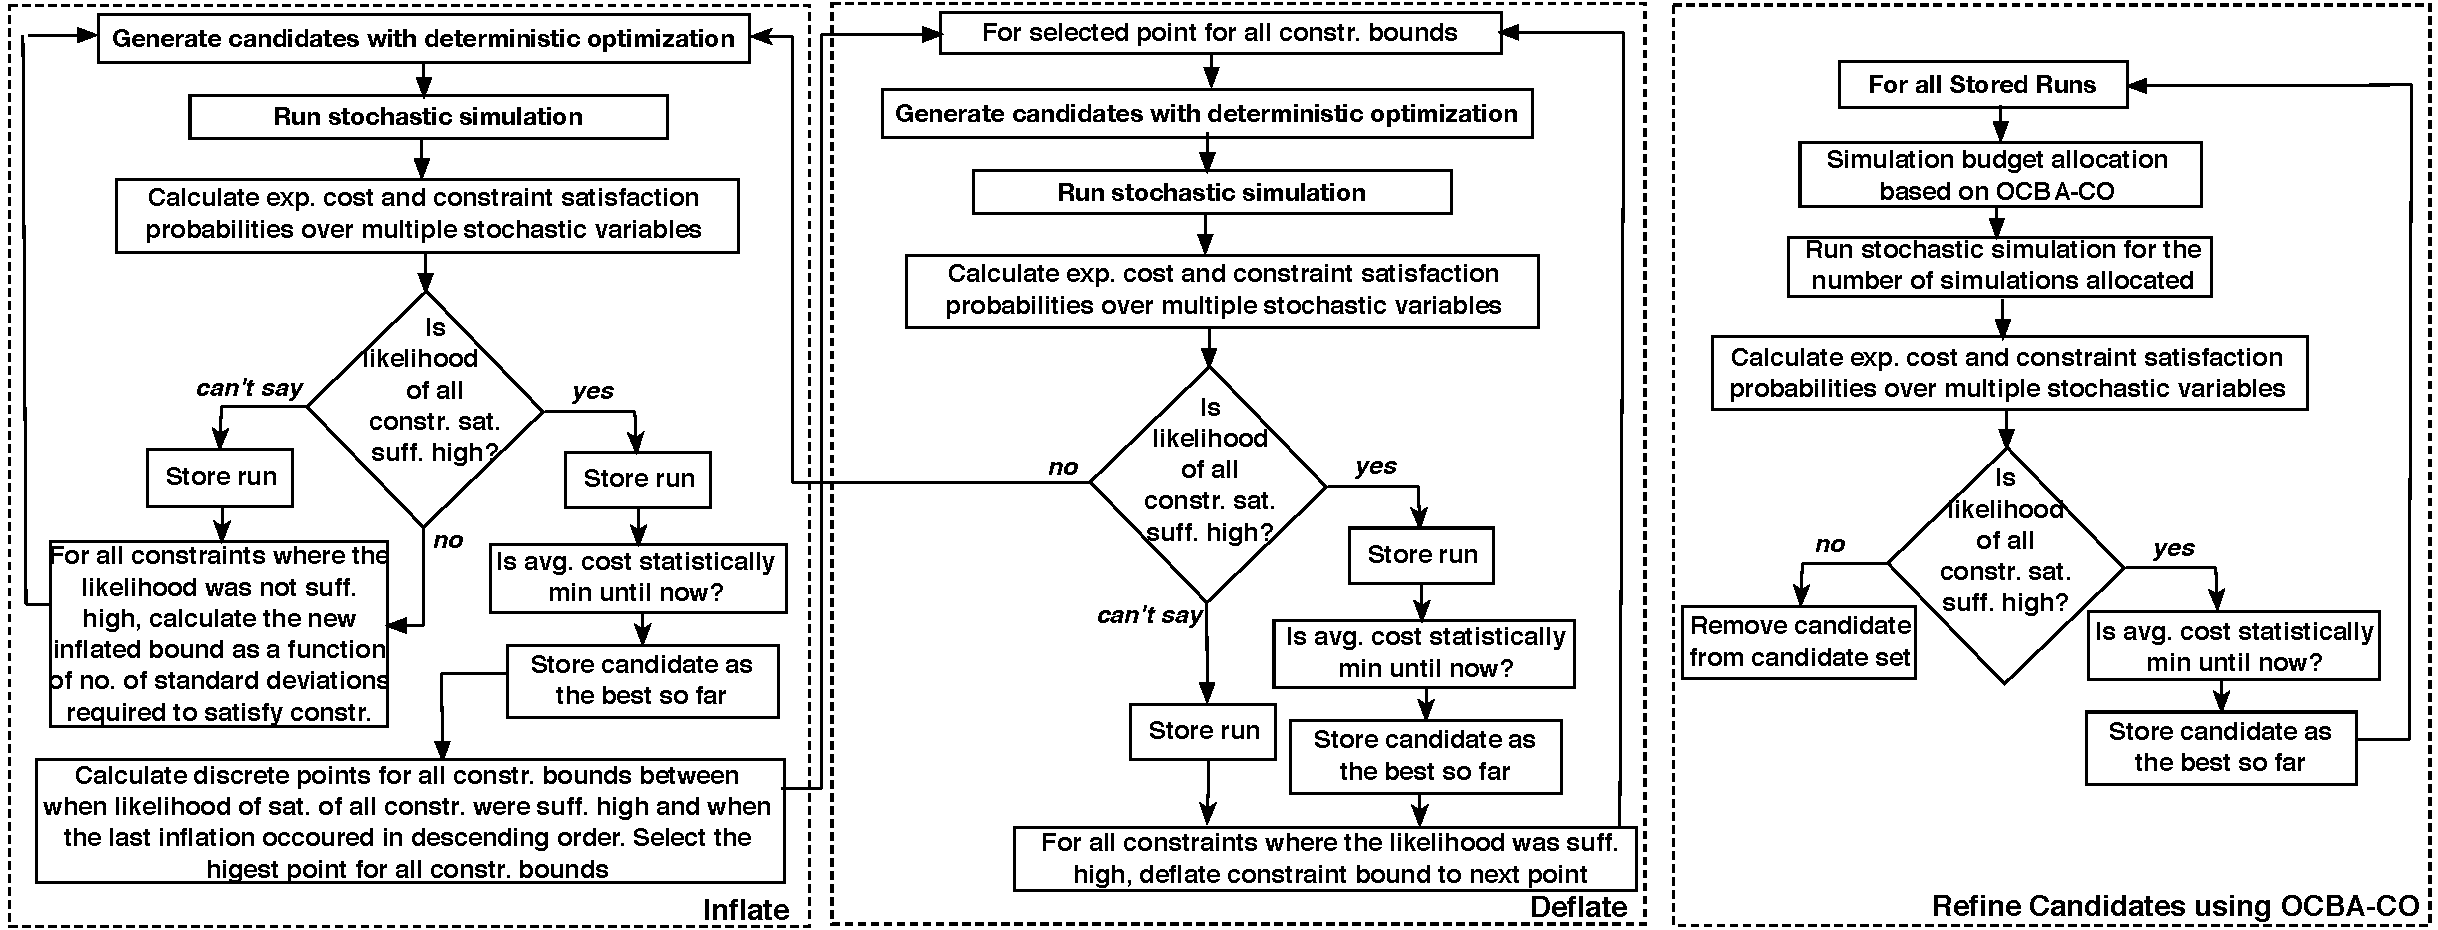
\includegraphics[width=\textwidth]{images/Algo_Full.pdf}
	\caption{Overview of g-SODA}
	\label{fig:algoOverview}       % Give a unique label
\end{figure}


\newcommand{\algoSODAm}{Algorithm 1}
\newcommand{\algoInflDefl}{Algorithm 2}
\newcommand{\algoPerfInfl}{Algorithm 3}
\newcommand{\algoInflate}{Algorithm 4}
\newcommand{\algoPerfDefl}{Algorithm 5}
\newcommand{\algoDeflate}{Algorithm 6}
\newcommand{\algoRefineCand}{Algorithm 7}
\newcommand{\algoExOCBA}{Algorithm 8}
\newcommand{\algoStochSim}{Algorithm 9}



An overview of g-SODA is shown in Fig. \ref{fig:algoOverview} and a corresponding pseudo code is given in \algoSODAm.~To generate a small set of candidate control settings, g-SODA performs deterministic approximations of the original stochastic problem. 
g-SODA achieves this by defining a deterministic computation $\mathbb{S}_0$ from the SCFA simulation $\mathbb{S}$ described in section \ref{sec:prob} by replacing every expression that uses a probability distribution $PD(\vec{P})$ with the expectation of that distribution. 
Thus the deterministic approximations \textit{cost$_0$}$(\vec{X})$, $m_{0,1}(\vec{X}),\dots,m_{0,k}(\vec{X})$ of \textit{cost}$(\vec{X})$, $m_1(\vec{X}),\dots,m_k(\vec{X})$, respectively can be expressed using $\mathbb{S}_0$.
To optimize this reduced problem, a deterministic optimization problem that approximates the stochastic optimization problem shown in equation \ref{eq:stochProb} is used as a heuristic. This deterministic optimization problem can be described as follows:
\begin{equation}
\label{eq:detApprox}
\begin{aligned}
& \underset{\vec{X}\in\vec{D}}{\text{minimize}}
& & \textit{cost}_0(\vec{X}) \\
& \text{subject to}
& & C(\vec{X}) \wedge \\
&&& m_{0,1}(\vec{X})\ge  \theta_1{'}\wedge\dots \wedge m_{0,k}(\vec{X})\ge  \theta_k{'} 
\end{aligned}
\end{equation}
where $\theta_1{'} \ge \theta_1,\dots,\theta_k{'} \ge \theta_k$ are conservative approximations of $\theta_1,\dots,\theta_k$. 

\begin{figure*}
	\begin{center}
	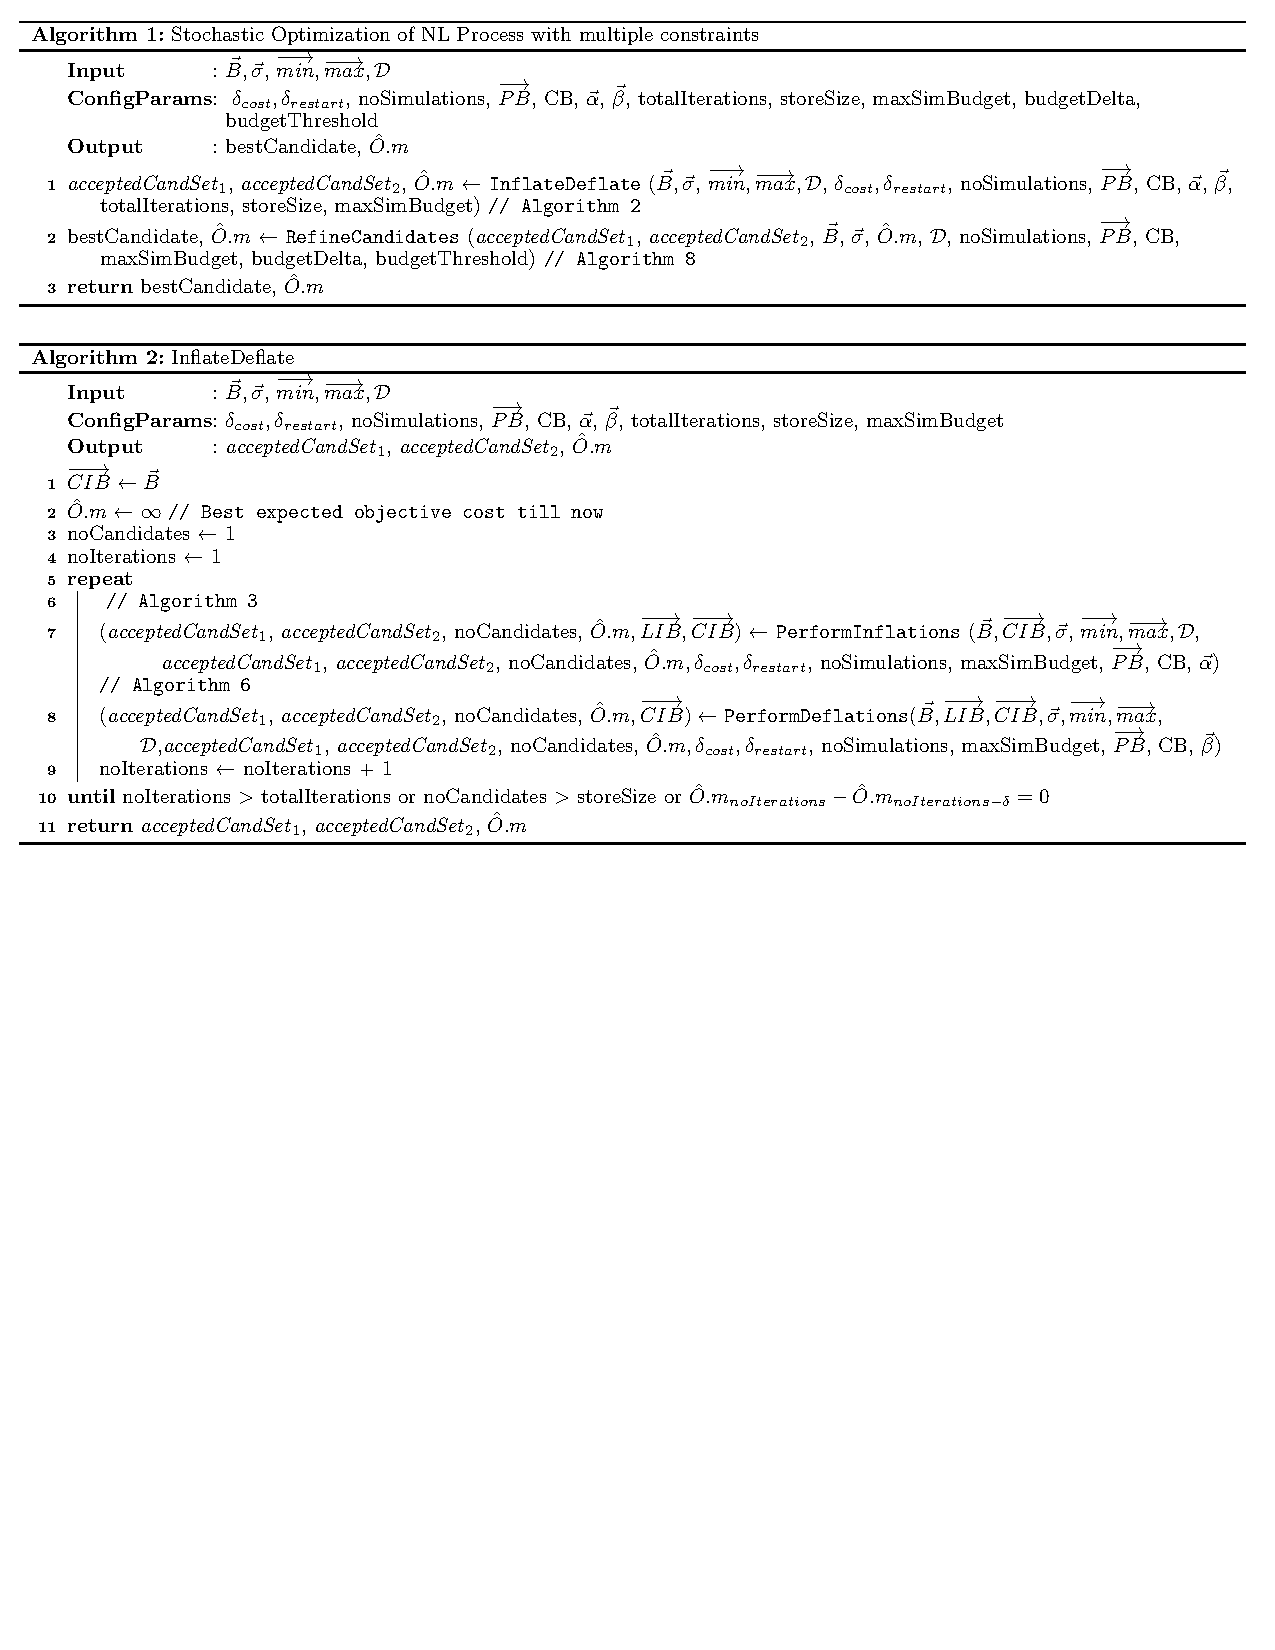
\includegraphics[width=.7\textwidth]{pseudoCode/Algo1-2.pdf}
	\end{center}

\end{figure*}
This deterministic approximation is performed iteratively such that the control settings found in the current iteration are more likely to satisfy the stochastic constraints with the desired probability than in the previous iterations. This is possible because of the \textit{inflate} phase (left box of Fig. \ref{fig:algoOverview}) and the \textit{deflate} phase (middle box of Fig. \ref{fig:algoOverview}) of g-SODA. 

The \textit{inflate} phase is intuitively trying to increase the bounds to satisfy the stochastic constraints with the desired probability. 
When the current candidate control settings do not generate any metric that satisfies its respective user-defined bound with a desired probability, this bound parameter itself is artificially inflated as a function of the number of standard deviations required so that the metric satisfies the bound with desired probability.
This inflation very quickly yields metrics that satisfy its respective user-defined bound. However, this may result in the metric overshooting the bound, which degrades the objective cost. 

To overcome this, in the \textit{deflate} phase, g-SODA scales the inflated bounds back by calculating the discrete points for all bounds between when the constraint was satisfied with sufficient probability and when the last inflation occurred.
 Deterministic approximations are run for this lower bound to check whether the updated metric still satisfies the user-defined bound with desired probability while yielding a better objective cost. 
 In this way, the \textit{inflate} and \textit{deflate} phases find a more optimum bound threshold for all stochastic constraints for which it can get the right balance between optimum cost and stochastic constraint satisfaction with desired probability.

After the iterative \textit{inflate} and \textit{deflate} procedure, more simulations may be needed to check if a promising candidate that currently is not a top candidate could be the optimal solution or to choose an optimal solution from multiple candidates. 
To resolve this, these candidates are further refined in the \textit{refineCandidates} phase (right box in Fig. \ref{fig:algoOverview}) where a number of simulations are allocated to each candidate as obtained from an optimal simulation budget allocation method. These simulations are run on these candidates to check if this produces a new optimal solution.

In this way, g-SODA uses model knowledge from the white box simulation code in \textit{inflate}, and \textit{deflate} phases, and optimal simulation budget allocation in \textit{refineCandidates} phase to provide optimal control settings of the non-linear processes with multiple stochastic constraints that a process operator can use on the manufacturing floor in a stochastic environment. The phases of g-SODA are explained in greater detail with the help of their pseudo-code in the subsections below.

\subsection{Inflate and Deflate Phase}
\label{ssec:inflDefl}
\begin{figure*}
\begin{minipage}[t]{.48\textwidth}
	\begin{center}
	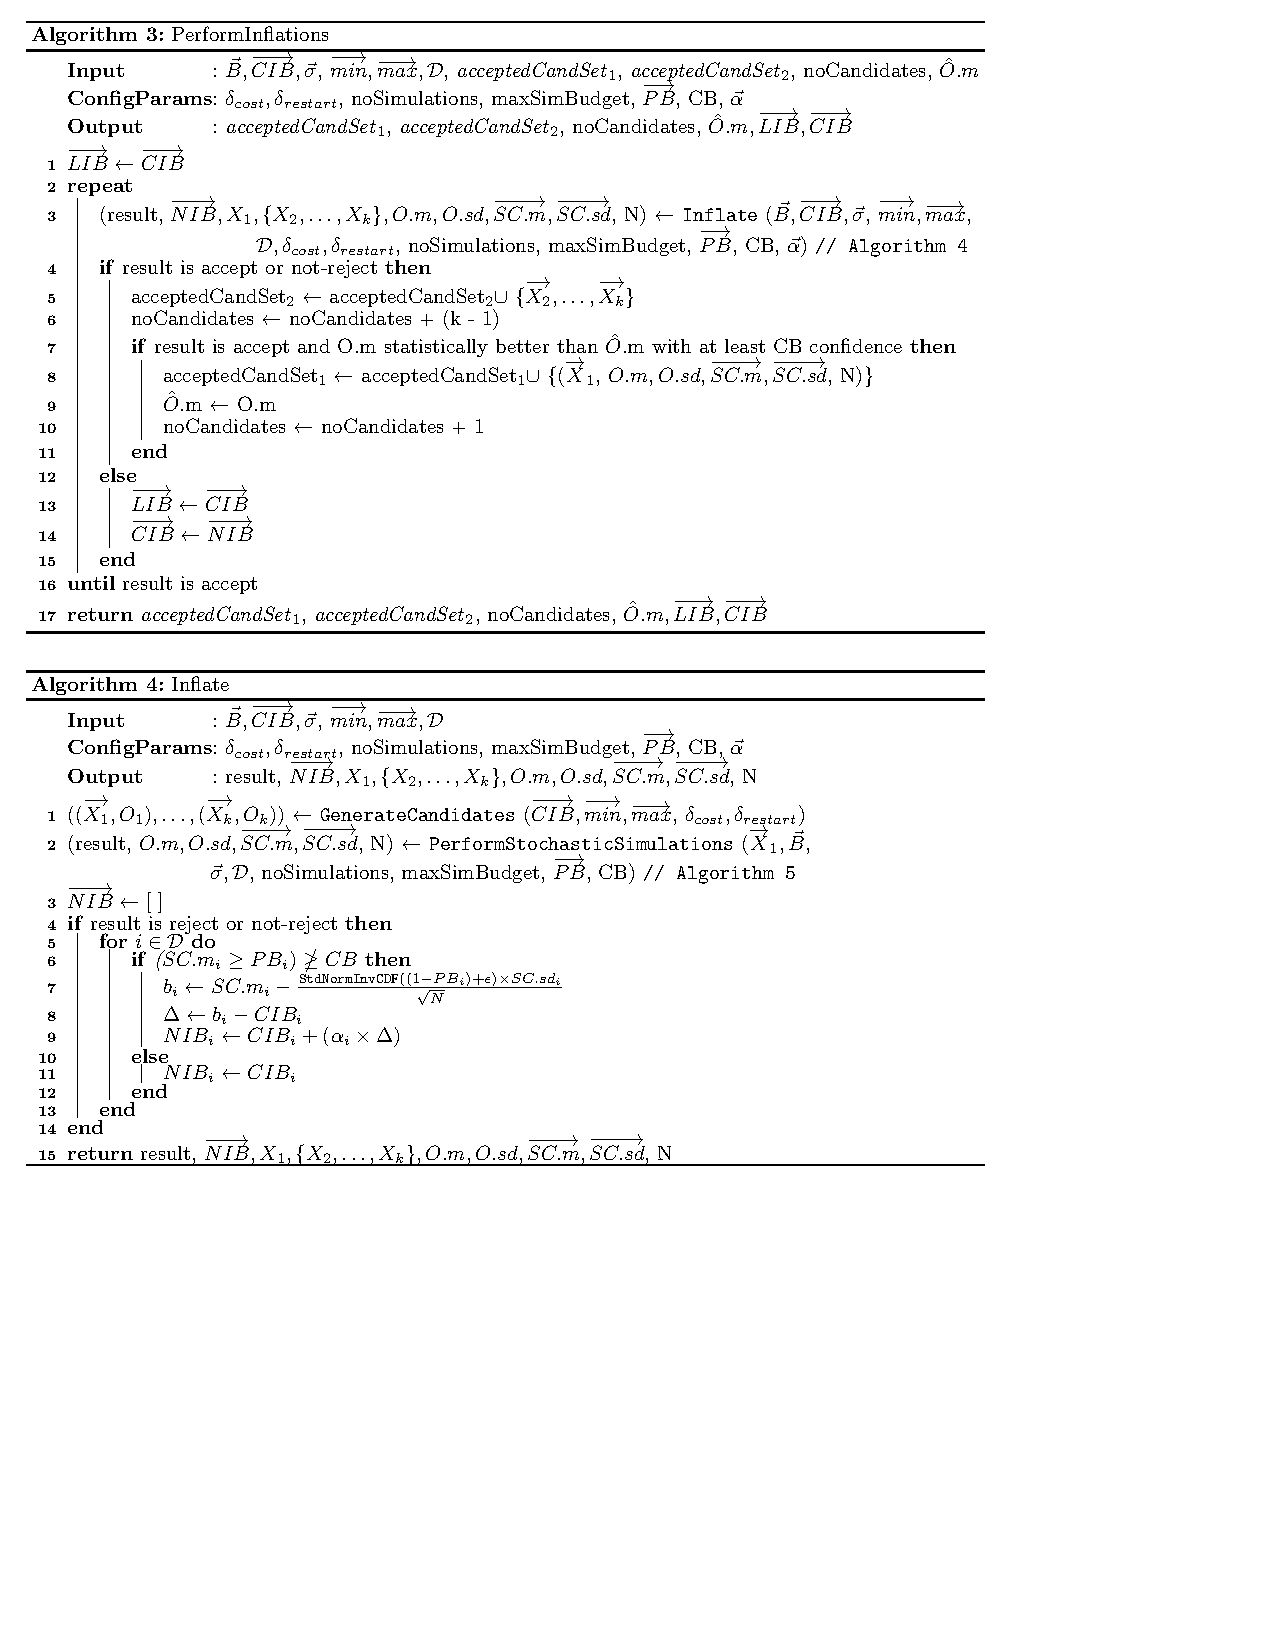
\includegraphics[width=1\textwidth]{pseudoCode/Algo3-4.pdf}
	\end{center}
\end{minipage}
\hfill
\begin{minipage}[t]{.5\textwidth}
		\begin{center}
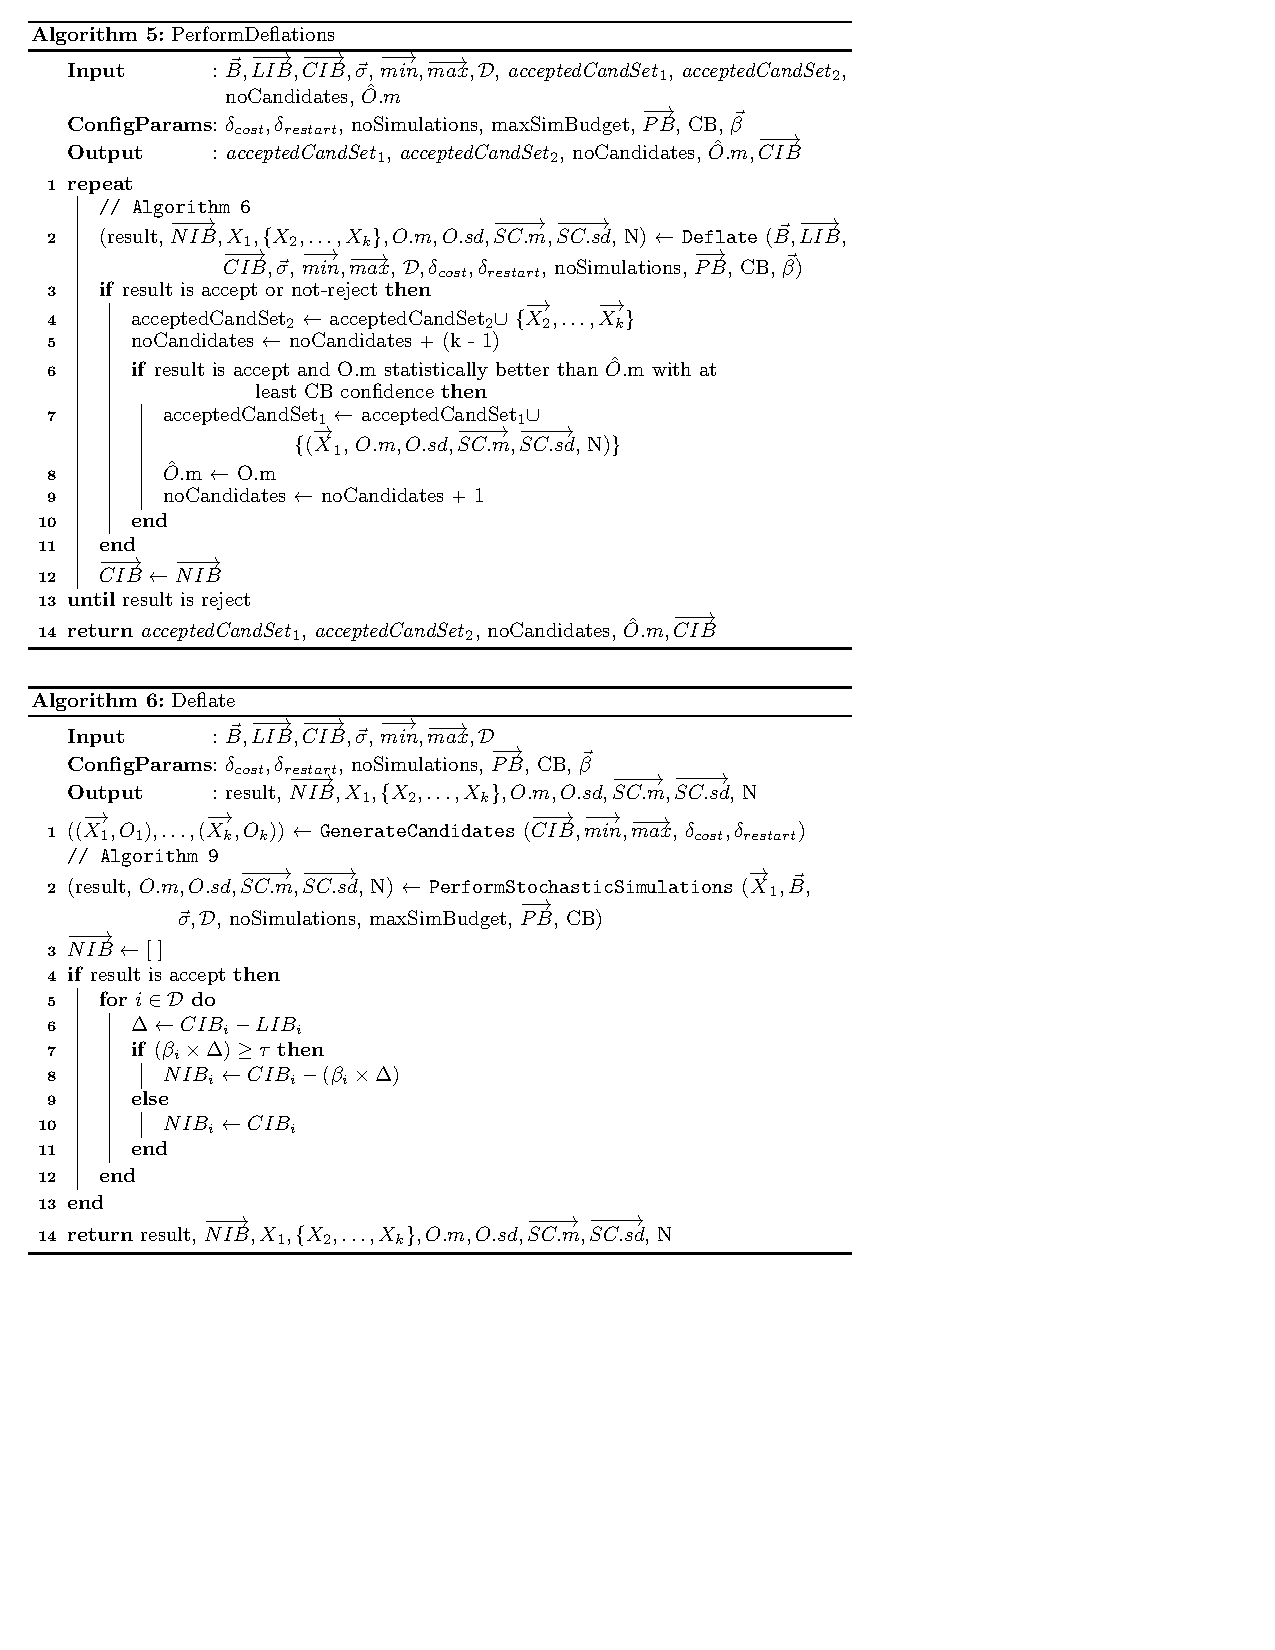
\includegraphics[width=1\textwidth]{pseudoCode/Algo5-6.pdf}
	\end{center}
\end{minipage}
\end{figure*}

The pseudo-code for the \textit{InflateDeflate} procedure is shown in \algoInflDefl~and it iteratively calls \textit{PerformInflations} and \textit{PerformDeflations} to perform deterministic approximation by inflating and deflating the bound parameters for a user defined budget or until there is no improvement in the objective cost ($\hat{O}.m$) for a certain number of iterations. The uniqueness of this procedure is that it is iterative and hence not only will the inflated bounds that satisfied the constraints with sufficient probability be the starting point for deflation but the bounds at which the deflation fails to satisfy any constraint with sufficient probability will be used to inflate from, thus yielding optimal solutions very early in the running of g-SODA.

The \textit{PerformInflations} procedure as shown in \algoPerfInfl~tries to iteratively find the inflated bounds for multiple constraints into $\overrightarrow{CIB}$ that can be used for deterministic approximation. The goal is that these inflated bounds will yield control settings when the problem in equation \ref{eq:detApprox} is solved and when these controls are used in the stochastic setting, the original constraints from the stochastic problem will be satisfied with sufficient probability.  
To achieve this, the \textit{PerformInflations} procedure calls \textit{Inflate} that performs one iteration of inflation as shown in \algoInflate. 

In the \textit{Inflate} procedure, first a number of candidate control settings with different objective costs are obtained by running a deterministic optimization with a constraint on the current bounds from $\overrightarrow{CIB}$ in the \textit{GenerateCandidates} procedure (\algoInflate~line 1). 
We adopt \textit{GenerateCandidates} procedure as is from \cite{GMU-CS-TR-2017-3} where random starting point are chosen for all the decision variables since the processes considered here have non-linear objectives that may not necessarily be convex. Then, the deterministic problem with the current bounds and different starting points are solved to generate different candidates with different control setting and objective costs. More information and pseudo-code of this procedure can be found in \cite{GMU-CS-TR-2017-3}.


The \textit{PerformInflations} procedure then calls the \textit{PerformStochasticSimulations} procedure as shown in \algoStochSim~that runs stochastic simulations on the candidate that yielded the least cost among the generated candidates and calculates the confidence of satisfaction of all the constraints as well as a verdict for this candidate that is returned back through the \textit{result} variable (\algoInflate~line 2). The \textit{result} variable can be \textit{accept}, when the probability of satisfaction of all the stochastic constraints are sufficiently high, \textit{reject}, when the probability of satisfaction of at least one of the stochastic constraint is not sufficiently high, and \textit{not-reject}, when \textit{accept} or \textit{reject} could not be decided for the number of simulations performed.

For all the constraints where the probability of satisfaction of the stochastic constraint is not sufficiently high, a new inflated bound is computed as a function of number of standard deviations required to satisfy the constraint with desired probability. The assumption here is that the population is normally distributed and the standard deviation remains approximately the same for the current bound and the inflated bound. Hence the inflated bound for the constraint is calculated by rearranging the terms in one-sample t-test (\algoInflate~lines 4-14). 
Finally, the \textit{result} variable, the new bounds ($\overrightarrow{NIB}$) and the generated candidates from the current iteration are returned from the \textit{Inflate} procedure (line 15). 
This returned information is then used in the \textit{PerformInflations} procedure to store the candidates and update the objective cost (\algoPerfInfl~lines 4-11). This inflation process continues until the new bounds calculated by the \textit{Inflate} procedure yields a \textit{result} of \textit{accept} when inflation of the bound parameters is no longer necessary (line 12-16).

%Deflation
The \textit{PerformDeflations} procedure as shown in \algoPerfDefl~tries to iteratively deflate the bounds that were inflated. These deflated bounds can be used for deterministic approximation. The goal here is that using these deflated bounds in the deterministic problem (equation \ref{eq:detApprox}) will yield control settings that will not only satisfy the original constraints from the stochastic problem with sufficient probability but do so with a better objective cost.  
To achieve this, the \textit{PerformDeflations} procedure calls the \textit{Deflate} procedure that performs one iteration of deflation as shown in \algoDeflate. 
In the \textit{Deflate} procedure, similar to the \textit{Inflate} procedure, the candidates are generated using the current bounds from $\overrightarrow{CIB}$ and stochastic simulations are run on these candidates to calculate the confidence of satisfaction of all the constraints and a verdict for the candidate in the \textit{result} variable (\algoDeflate~lines 1-2). 
If the \textit{result} is \textit{accept} the interval between the current bound and the bound at which the last inflation occurred is divided by a constant amount from $\vec{\beta}$ (lines 4-13). 
Finally, the \textit{result} variable, the new bounds ($\overrightarrow{NIB}$) and the generated candidates from the current iteration are returned from the \textit{Deflate} procedure (line 14). 
This returned inormation is then used in the \textit{PerformedDeflations} procedure to store the candidates and update the objective cost (\algoPerfDefl~lines 3-9). This deflation process continues until the new bounds calculated by the \textit{Deflate} procedure yields a \textit{result} of \textit{reject} when deflation of bounds is no longer useful to  generate better candidates (line 12-13).





\subsection{Candidate Refinement Phase}
\label{ssec:refineCand}

\begin{figure*}
	\begin{minipage}{\textwidth}
		\begin{center}
		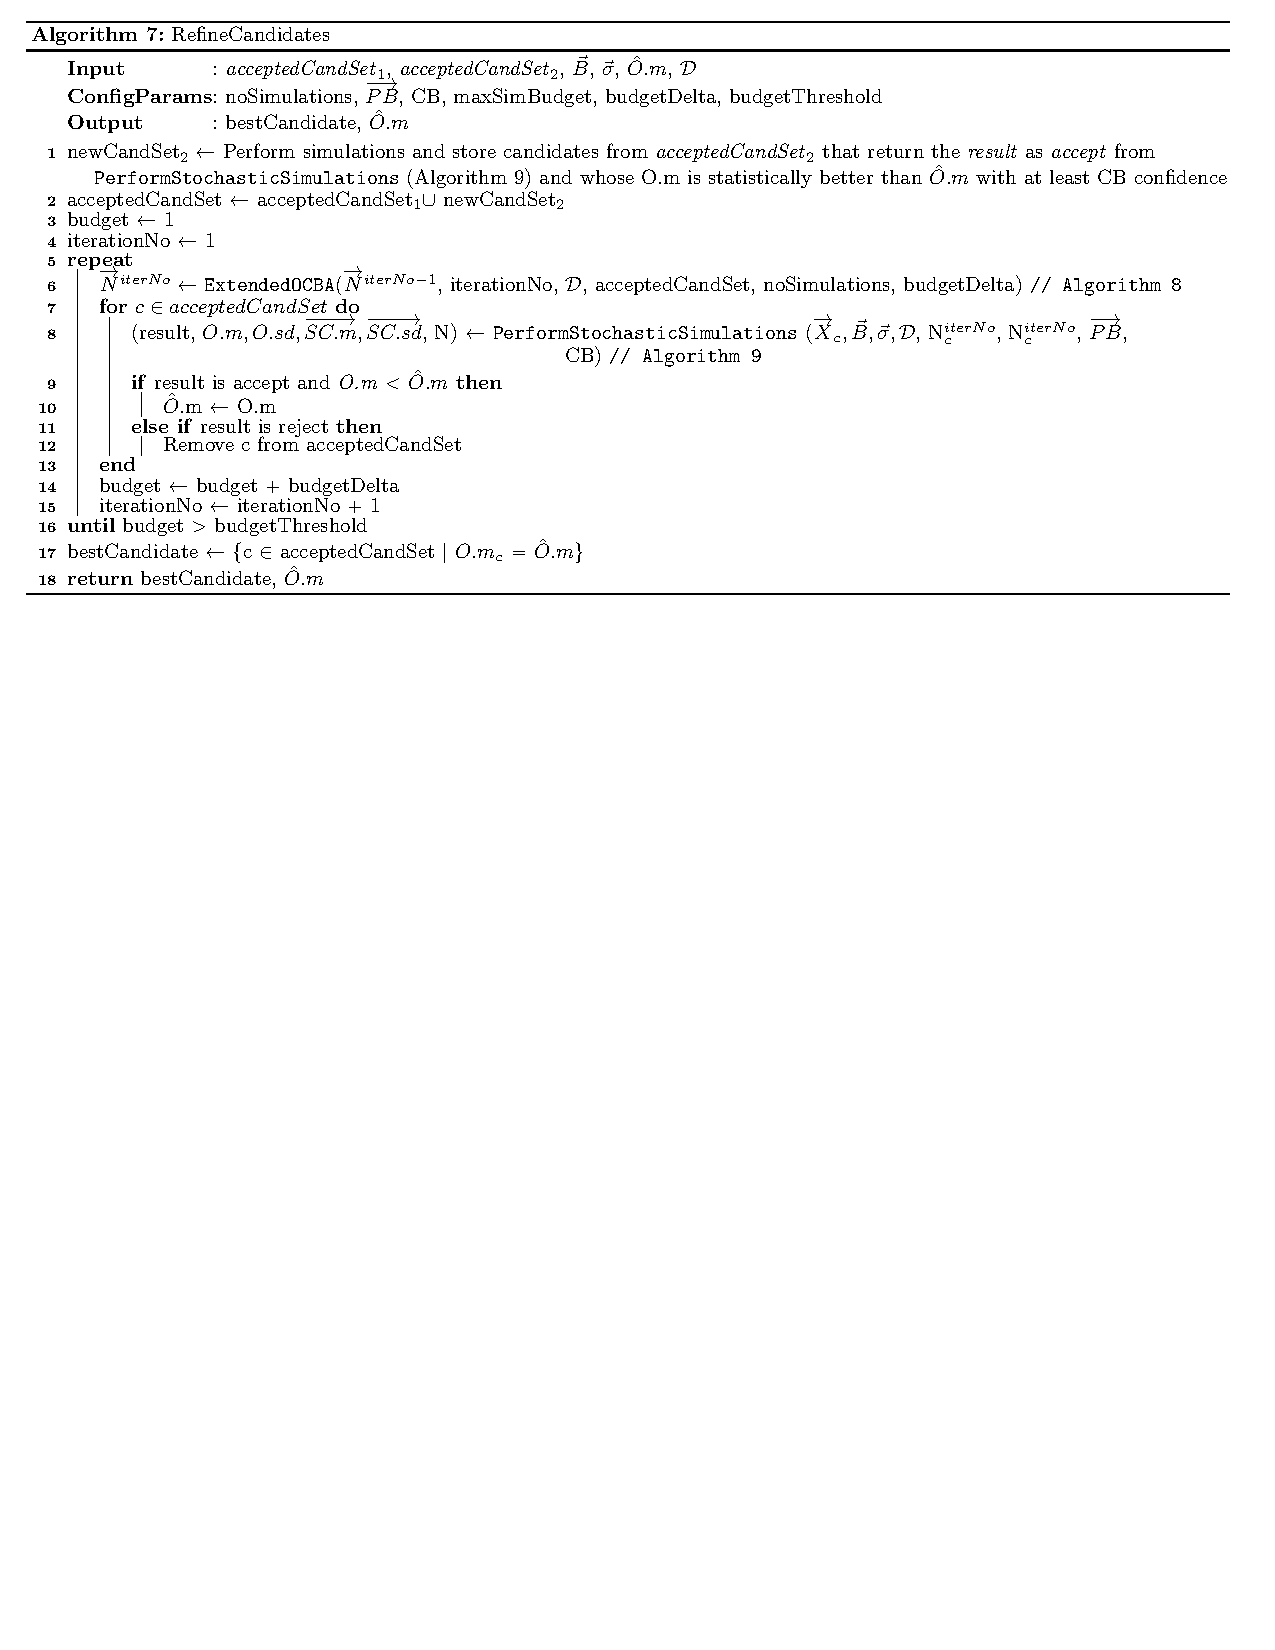
\includegraphics[width=.7\textwidth]{pseudoCode/Algo7.pdf}
	\end{center}
	\end{minipage}
	\vspace{1em} % add some whitespace after the first figure
	
	\begin{minipage}[b]{0.54\textwidth}
		\begin{center}
		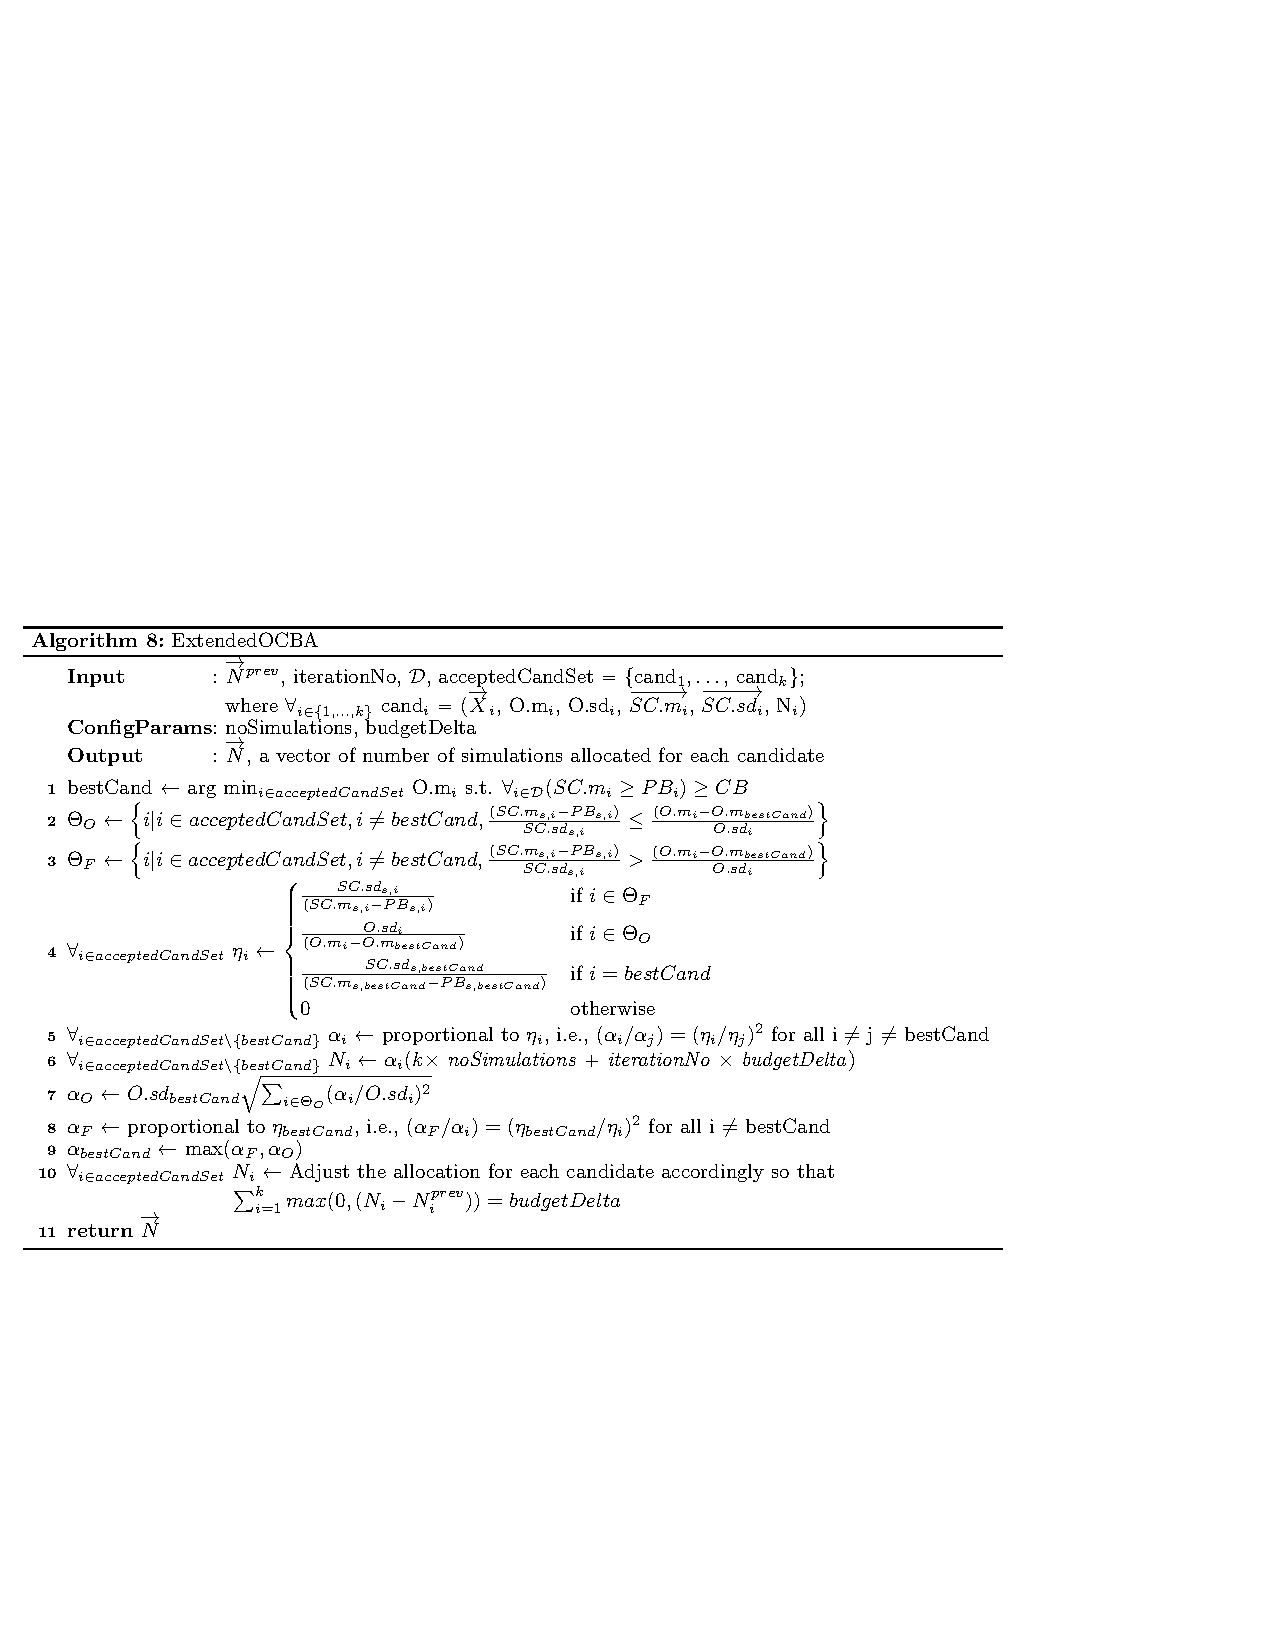
\includegraphics[width=1\textwidth]{pseudoCode/Algo8.pdf}
	\end{center}
	\end{minipage}
	\hfill
	\begin{minipage}[b]{0.45\textwidth}
		\begin{center}
		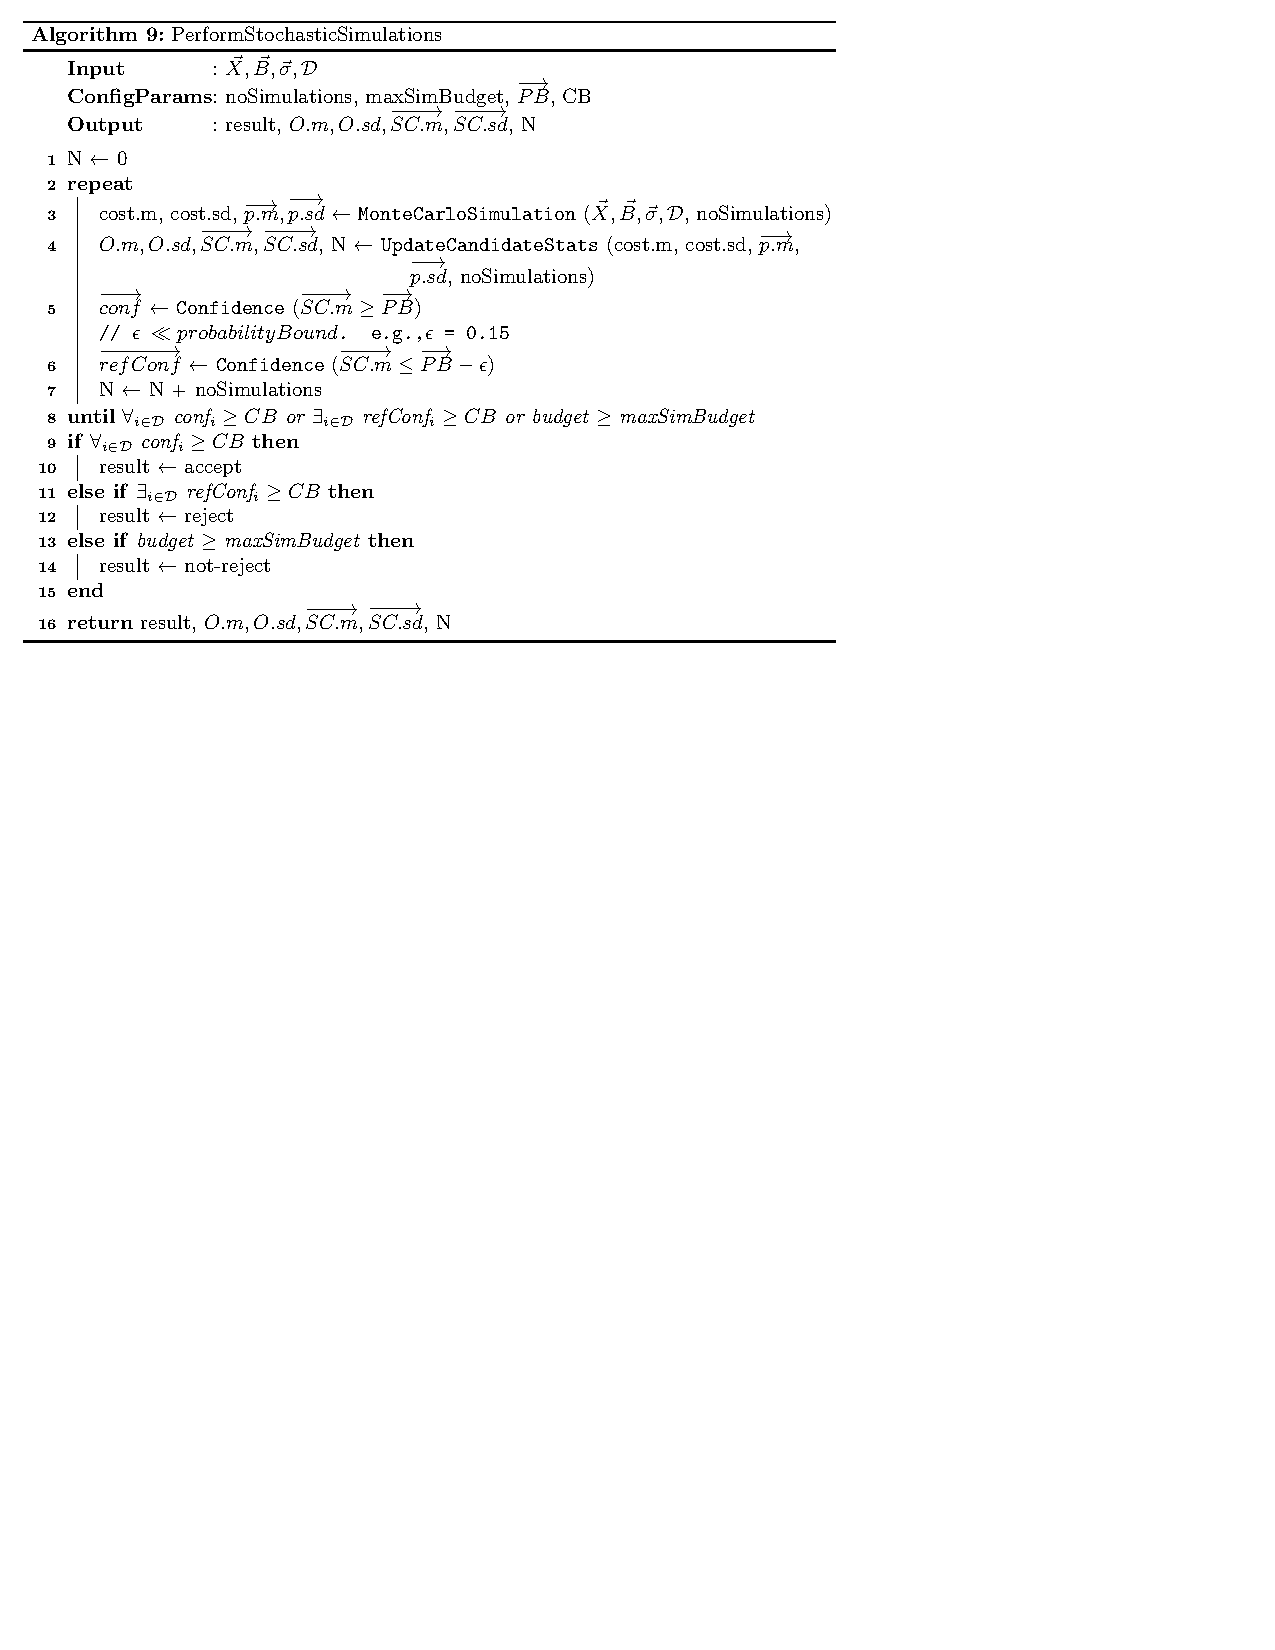
\includegraphics[width=1\textwidth]{pseudoCode/Algo9.pdf}
	\end{center}
	\end{minipage}
\end{figure*}

After generating the candidate sets using deterministic approximations, g-SODA refines these candidates by running Monte Carlo simulations on them in this phase. 
To maximize the likelihood of selecting the best candidate, i.e., candidate with the least cost and sufficient probability of satisfaction of all constraints, this phase uses the Optimal Computing Budget Allocation method for Constraint Optimization (OCBA-CO) \cite{Lee2012OCBACO} to allocate some delta budget among the candidates so that the greatest fraction of the budget is allocated to the most promising candidates in the candidate set. In each iteration of this phase, the allocated simulation budget is run on the candidates.
In each subsequent iteration, OCBA-CO can use the updated estimates to find new promising candidates and allocate a greater fraction of the delta budget to them to check if these candidates can be further refined.

The pseudo-code for the \textit{RefineCandidates} procedure is given in \algoRefineCand. 
In this procedure, first, simulations are run on any candidates for which there are no base statistic, i.e, candidates on which simulations was not run in the inflate and deflate phase. Those candidates that return the result of \textit{accept} and whose objective cost is statistically better than the best objective cost so far are stored for further consideration (\algoRefineCand~lines 1-2).
Then, this phase uses the \textit{ExtendedOCBA} procedure, which is based on OCBA-CO, to iteratively allocate a fraction of the delta budget among the candidates (line 6).
Then, stochastic simulations are run for the allocated number of simulations for each candidate (line 8).
If the calculated verdict for the candidate (\textit{result}) is \textit{accept} and if the cost is further minimized, then the best cost is updated (lines 9-10).
On the other hand, if the \textit{result} is \textit{reject}, then the candidate is removed from further consideration (lines 11-12).
This iteration of budget allocation and simulation refinement continues until some maximum amount of simulation budget is depleted.

The pseudo-code for the \textit{ExtendedOCBA} based on OCBA-CO procedure is given in \algoExOCBA.
This procedure allocates a greater fraction of the delta budget to candidates that have the highest likelihood of being the best candidate or near the best candidate. 
In this case, the best candidate is the one with the best cost with sufficient confidence of satisfaction of all the stochastic constraints (line 1).
This procedure creates two sets for the non-best candidates: $\theta_O$ where optimality of cost objective is a more dominant feature among the candidates and $\theta_F$ where probability of a significant constraint is a more dominant feature among the candidates (lines 2-3). 
Then, the noise-to-signal ratio of each candidate is obtained (line 4).
Finally, the number of allocated simulations is obtained proportional to their noise-to-signal ratio (lines 5-10). 
More details about the OCBA-CO algorithm can be obtained from \cite{Lee2012OCBACO}.

\section{Experimental Study}
\label{sec:expResults}

\begin{figure}
	\begin{center}
		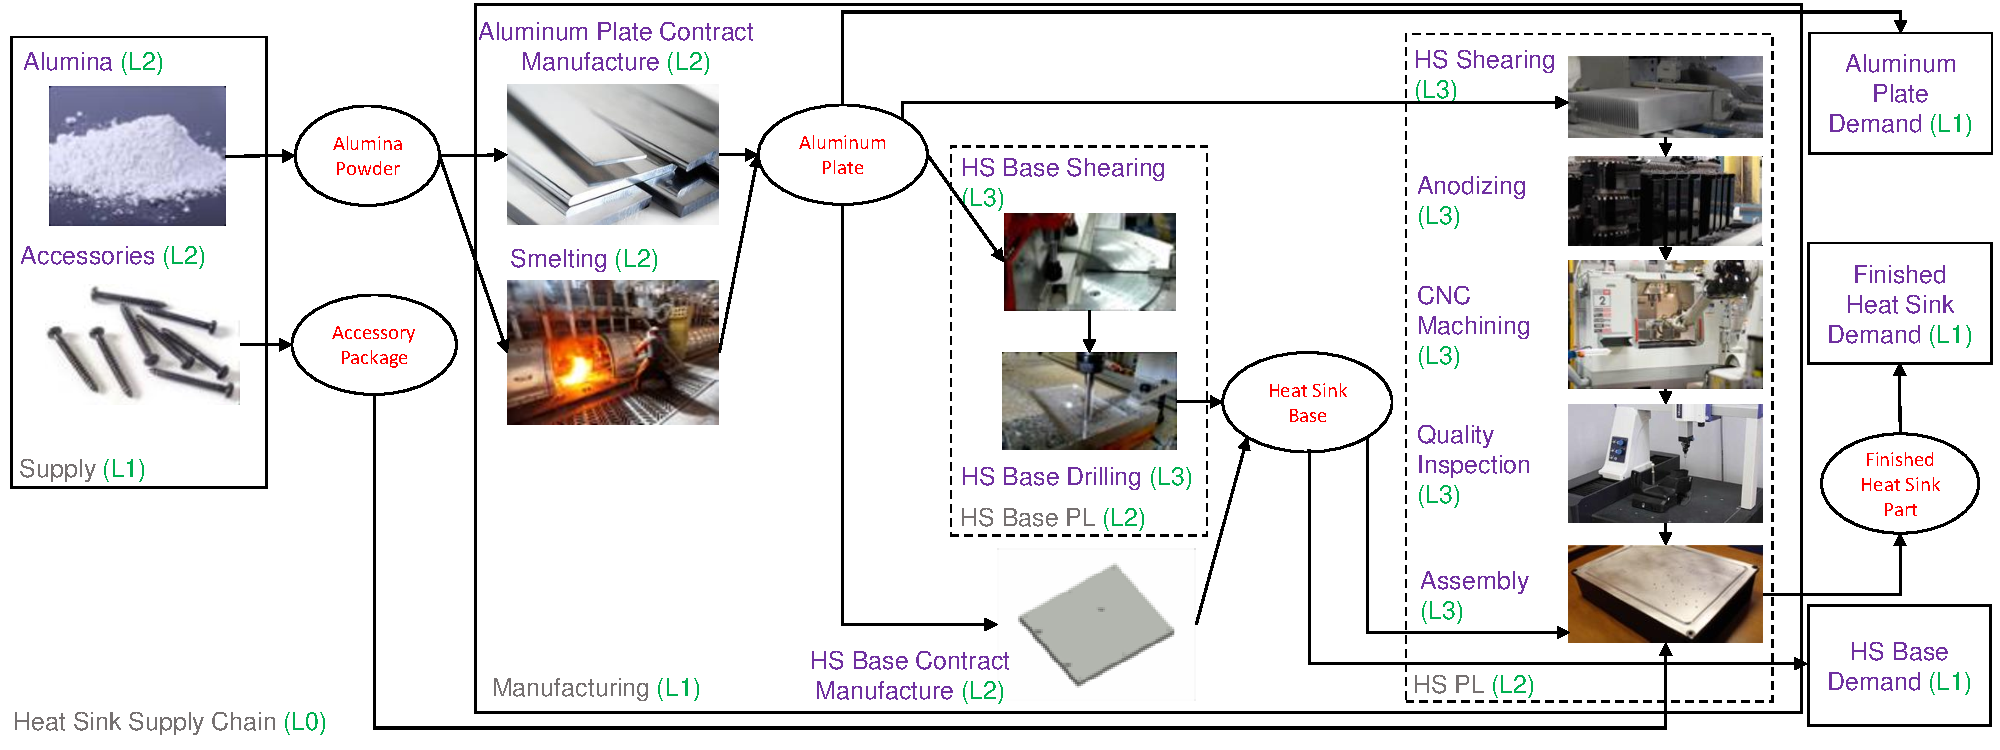
\includegraphics[width=0.7\textwidth]{images/HeatSink_contractSN.pdf}
		\caption{Graphical representation of the Heat-Sink Production Process (HSPP)}
		\label{fig:heatsinkSC}       % Give a unique label
	\end{center}
\end{figure}

This section describes the experimental study that was conducted to evaluate g-SODA in terms of its quality of objective cost and rate of convergence as compared to four metaheuristic simulation-based optimization algorithms. 
In this study a real-world use-case of the Heat Sink Production Process (HSPP) is considered.
The graphical representation for the HSPP  is shown in Fig. \ref{fig:heatsinkSC}.
The production process can be described as a composition of three sub-processes of \textit{supply}, \textit{production}, and \textit{demand}. 
The \textit{supply} sub-process further contains the suppliers of the raw materials for the heat-sink part, which includes suppliers of \textit{aluminum}, \textit{heat-sink case} and \textit{accessories} such as screws, and bolts. 
The production sub-process contains processes that will transform the input raw materials into the output heat-sink part. 
To do this, the raw material of \textit{aluminum} is first cut using a \textit{cutting/shearing} process. Then, the cut aluminum is sent to a \textit{CNC machining} process that uses the \textit{milling} and \textit{drilling} sub-processes to mill and drill on the cut aluminum part to produce the raw heat-sink part. Then, this raw part goes through the \textit{washing and finishing} process, after which it is inspected for defects and accuracy in the \textit{quality inspection} process. Finally, this inspected part is assembled together with the \textit{heat-sink case} using the \textit{accessories} in the \textit{assembly} process.
The last sub-process is a virtual process for \textit{demand}, which contains processes that dictate the minimum number of aluminum plate, finished Heat Sink, and Heat Sink Base to be produced so as to satisfy either the customer demand or foretasted sales. 


To conduct the experimental study, first the SCFA simulation of HSPP is written in JSONiq. An overview of the SCFA simulation for a production process in given in \cite{GMU-CS-TR-2017-3}.  The code for g-SODA is written in Java. The deterministic approximations for g-SODA are performed using a system that automatically converts the SCFA simulation of HSPP into a deterministic optimization problem, which is a deterministic abstraction of the original SCFA simulation. Discussing the code of the SCFA simulation for HSPP and the system that performs its automatic conversion is outside the scope of this paper. But more details about an initial realization of these can be found in \cite{Brodsky2016ieeebd,Brodsky2017ieeebd}.

For the comparison algorithms, we used the jMetal package, which is an object-oriented Java-based framework for multi-objective optimization with metaheuristics \cite{jMetal}. The algorithms chosen for comparison include Nondominated Sorting Genetic Algorithm 2 (NGSA2) \cite{ngsa2}, Indicator Based Evolutionary Algorithm (IBEA) \cite{ibea}, Strength Pareto Evolutionary Algorithm 2 (SPEA2) \cite{spea2}, and Speed-constrained Multi-objective Particle swarm optimization (SMPSO) \cite{NDG09}.
All these algorithms use the SCFA of HSPP to perform the computation of the cost and other stochastic metrics as well as the feasibility constraints. The cost and constraint satisfaction information is then used by the jMetal algorithms to further increase or decrease the control settings using heuristics.

We ran g-SODA was in two different settings. 
In the first setting, g-SODA was run for one day with 5,000 iterations of \textit{InflateDeflate}. In the second setting, g-SODA was run for approximately 72 hours (three days) with 10,000 iterations of \textit{InflateDeflate}. There were 22 decision variables and 21 stochastic constraints in the stochastic optimization problem over HSPP. The probability bound and the confidence bound for all stochastic constraints were set to 0.95 and 99\% respectively. Additionally, all production processes in HSPP were stochastic due to noise added to their controls. This noise has a mean of 0 and standard deviation between 1.8 to 2.8. 
Finally, the demand for aluminum plate, finished Heat Sink, and Heat Sink Base were set to 8, 4, and 6 respectively.
The comparison algorithms were also run with the same (relevant) parameters.

\begin{figure}
	\begin{minipage}{.5\textwidth}
	\begin{center}
	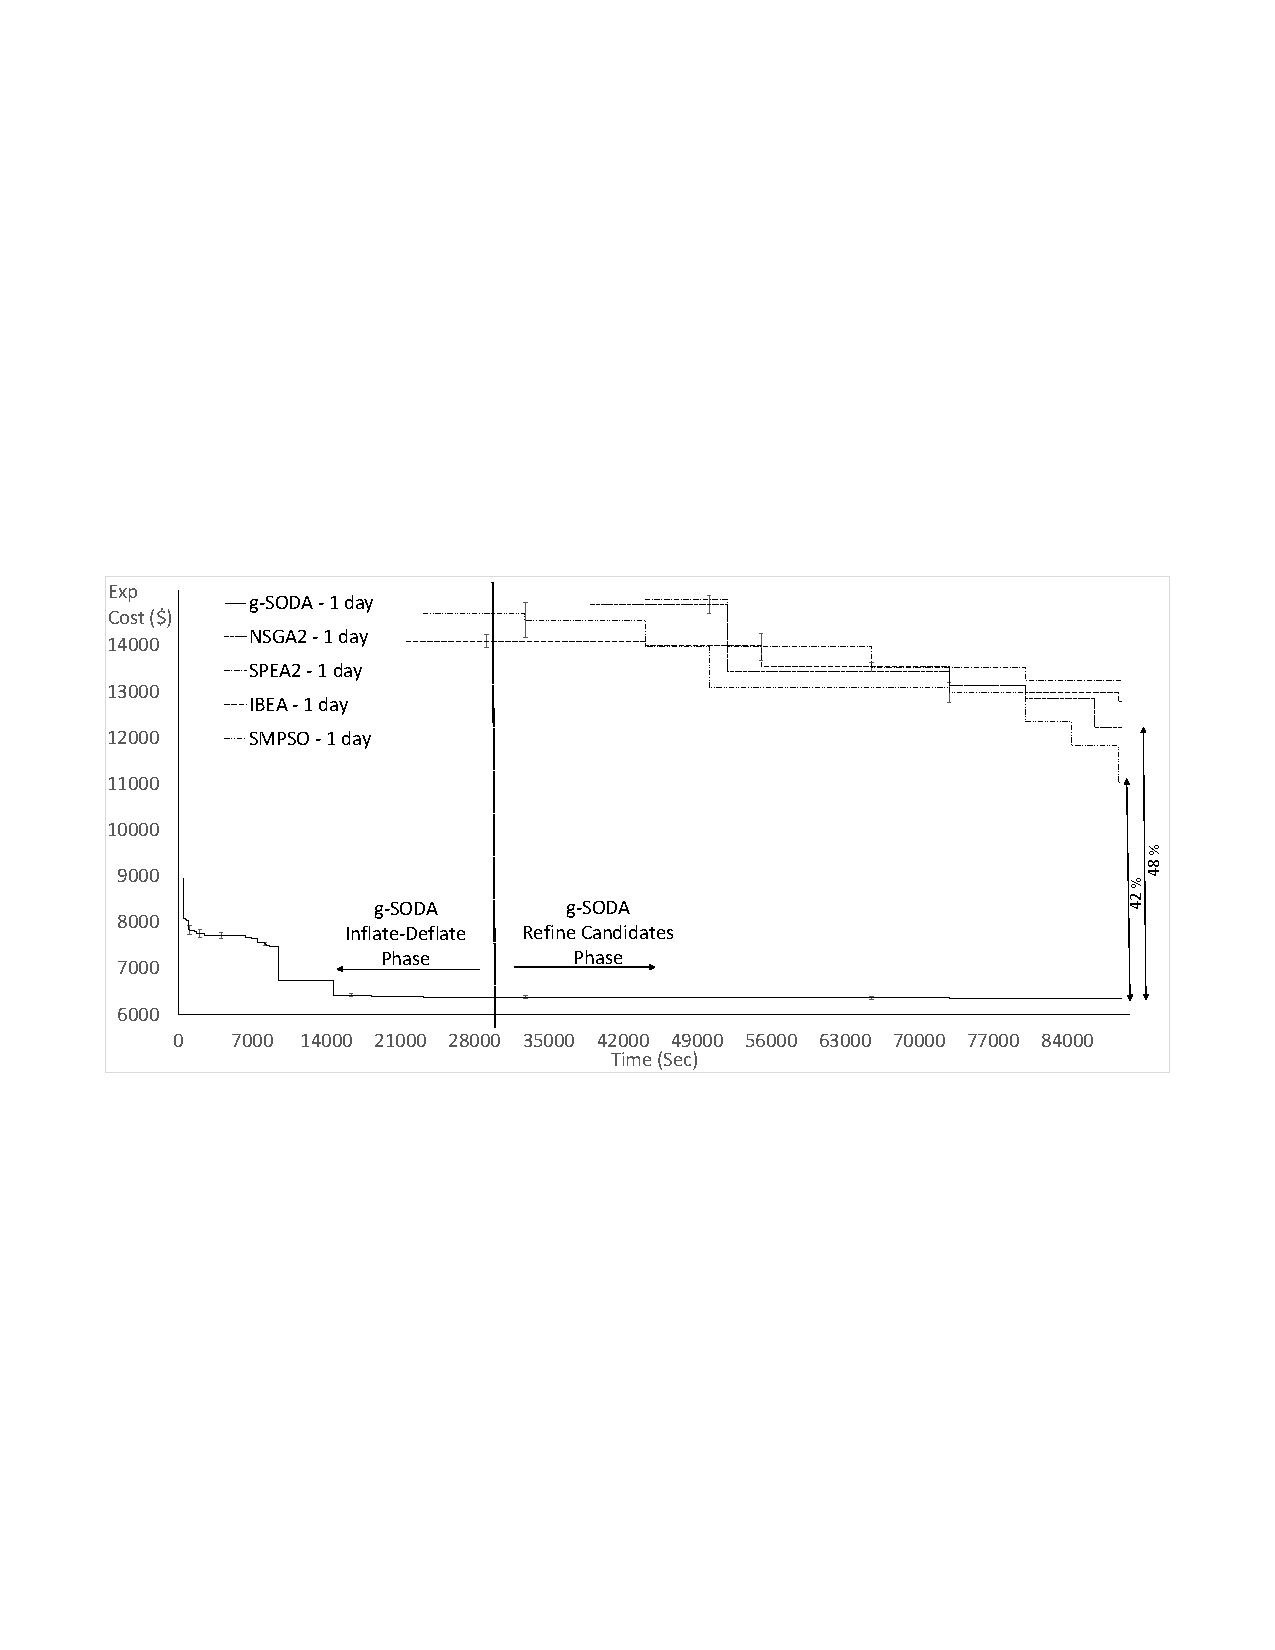
\includegraphics[width=\textwidth]{images/sodavsjmetal1day.pdf}
	\caption{Estimated average cost for the elapsed time (max runtime = one day) (x-axis in normal scale}
	\label{fig:GraphsForTime_24hours}       % Give a unique label
\end{center}
\end{minipage}
%	\vspace{.5em} % add some whitespace after the first figure
\hfill
\begin{minipage}{.5\textwidth}
	\begin{center}
	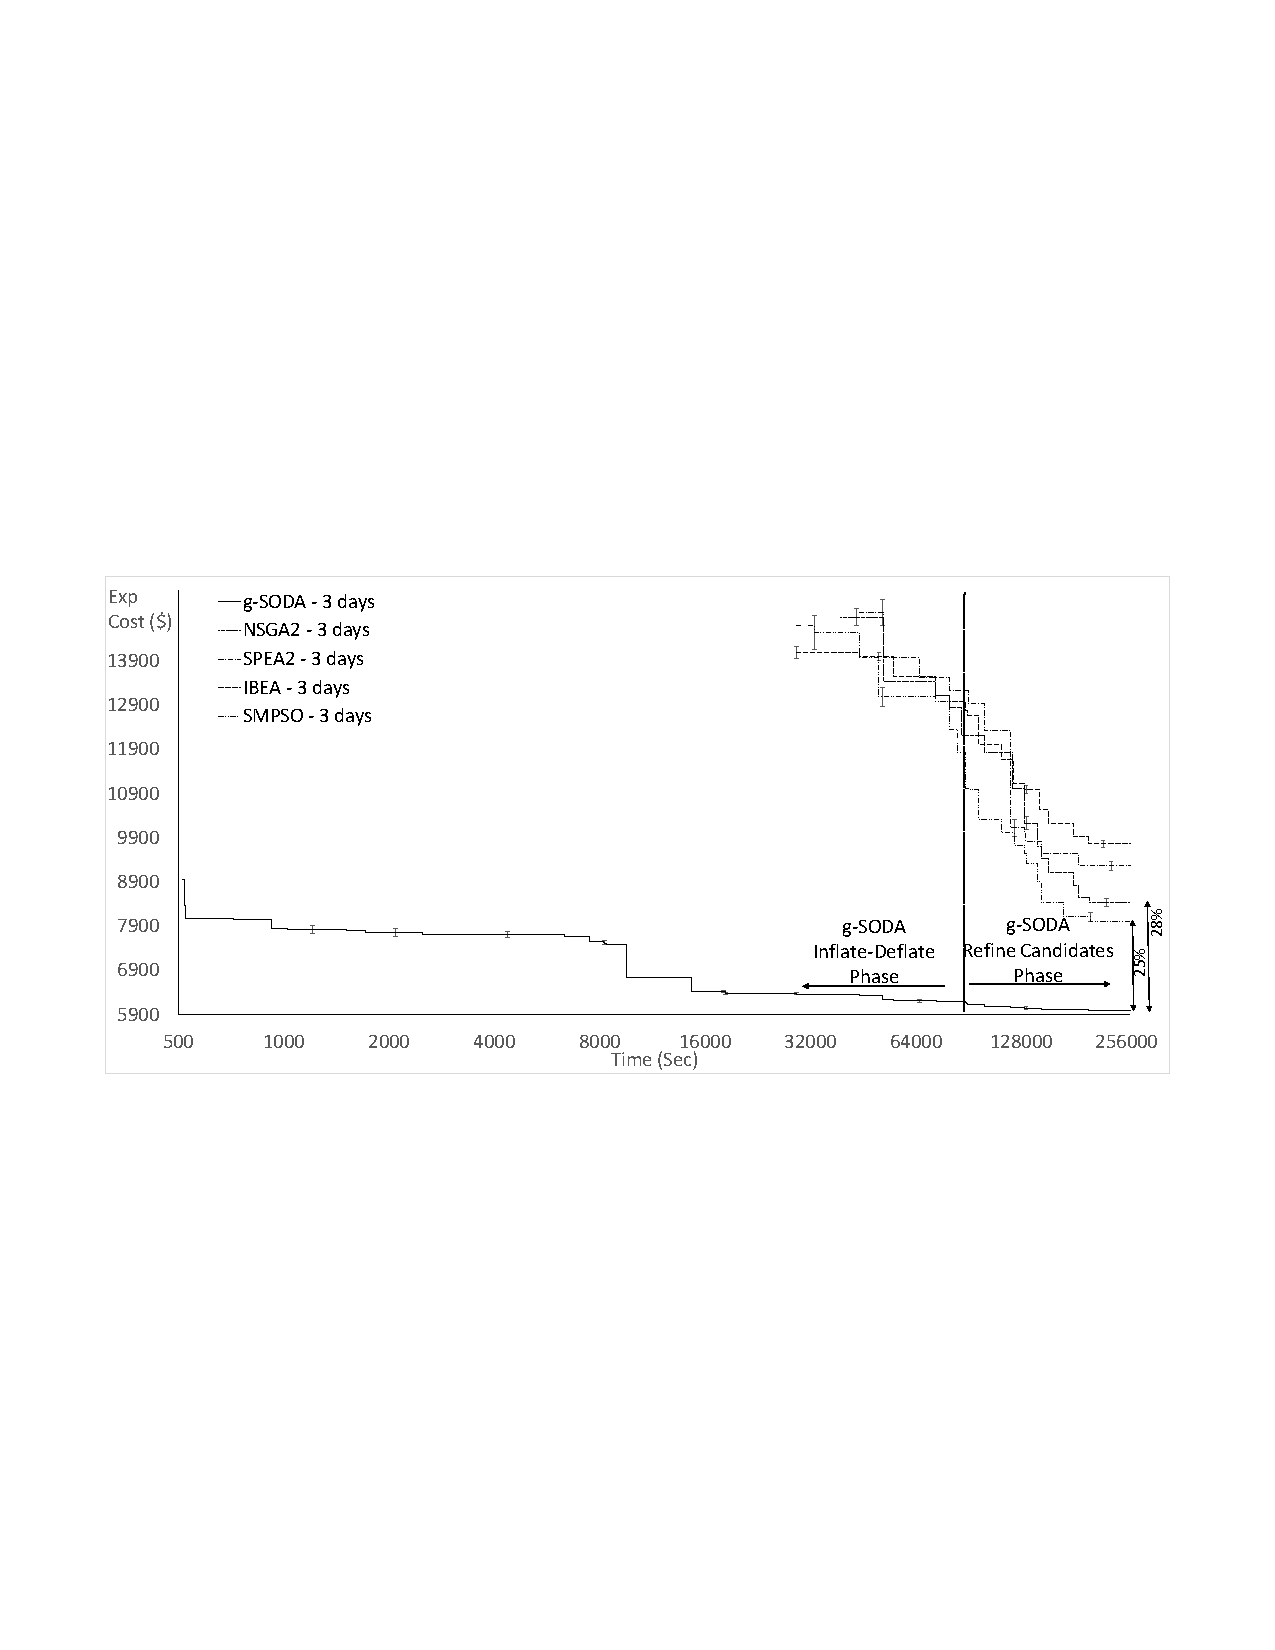
\includegraphics[width=\textwidth]{images/sodavsjmetal3day.pdf}
	\caption{Estimated average cost for the elapsed time (max runtime = three days) (x-axis in log-scale)}
	\label{fig:GraphsForTime_3days}       % Give a unique label
\end{center}
\end{minipage}
\end{figure}

%SODA vs JMetal
The data collected from the experiments include the estimated average costs achieved at different elapsed time points for g-SODA in two settings and all the comparison algorithms. 
Fig.~\ref{fig:GraphsForTime_24hours} shows the estimated average costs achieved after one day whereas Fig. \ref{fig:GraphsForTime_3days} shows the estimated average costs achieved after about three days. Each experiment was run multiple times and 95\% confidence bars are included around the mean at certain elapsed time point in both figures. 

It can be observed that both settings of g-SODA perform better than the comparison algorithms initially. This is because g-SODA uses deterministic approximation to reduce the search space of potential candidates quickly whereas the competing algorithms start at a random point in the search space and need a number of additional iterations (and time) to even find candidates that satisfy all the stochastic constraints with sufficient probability. 

As time progresses, SODA in both settings is able to achieve much better expected cost in the \textit{inflateDeflate} phase itself whereas the comparison algorithms proceed to reduce the gap to g-SODA very slowly.
Hence, we claim that g-SODA is able to converge quicker toward the points close to the (near) optimal solution found at the end of the algorithm. This is because g-SODA uses heuristics in the \textit{inflate} and \textit{deflate} phases that reduce the search space quickly, which allows g-SODA to quickly converge toward a more promising candidate. 

Additionally, g-SODA is able to reduce the cost further in the \textit{RefineCandidates} phases with OCBA-CO simulation budget allocation. Due to this, it is observed that the solutions found by g-SODA at the end of the experiment are much better than those found by the competing algorithms.
After one day, the expected cost found by g-SODA was 42\% better than the nearest comparison algorithm (SMPSO) (see Fig. \ref{fig:GraphsForTime_24hours}). After three days, the advantage for g-SODA over the nearest comparison algorithm (SMPSO) reduces to 25\% and that to the second best algorithm (NSGA2) is 28\% (see Fig. \ref{fig:GraphsForTime_3days}). 
%This is not surprising since SMPSO and NSGA2 use strong meta-heuristics and given enough time such algorithms will eventually converge toward the (near) optimal solution found by g-SODA. Although, it should be noted from Fig. \ref{fig:GraphsForTime_3days} that g-SODA reaches close to the optimal solution found at the end much more quickly than its competition. Also, since the x-axis in Fig. \ref{fig:GraphsForTime_3days} is in log scale, it should be noted that out of the total experiment time of about 259,200 sec, the other algorithms stop improving at around 180,911 sec whereas g-SODA continues to improve for a longer time (until about 210,562 sec) due to a good collection of candidates from the \textit{InflateDeflate} phase and performing simulation refinements using an optimal budget allocation scheme of OCBA-CO in \textit{RefineCandidates} phase. 
We also ran the Tukey-Kramer procedure for pairwise comparisons of correlated means on all six algorithm types. By doing so, we confirmed that g-SODA was indeed better than the other algorithms when the experiment ended.

Although this experimental study compares g-SODA's performance against four popular metaheuristic simulation-based optimization algorithms, it may be useful to compare g-SODA's performance to methods that solve the same problem using techniques that typically extract the mathematical structure of the problem using black box simulations and utilize this structure to perform deterministic approximations. 
Such a comparison may result in a better understanding of how g-SODA performs against similar but known to be less efficient approaches than g-SODA. 
But such a comparative study is outside the scope of this paper and we defer this study to our future work.

\section{Conclusion and Future Work}
\label{sec:conclusion}

This paper presents an efficient stochastic optimization algorithm called g-SODA for the problem of finding process controls of a steady-state production processes that minimize the expectation of cost while satisfying multiple deterministic and stochastic feasibility constraints with a given high probability. 
This algorithm is based on performing (1) a series of deterministic approximations to produce a candidate set of near-optimal control settings for the production process, and (2) stochastic simulations on the candidate set using optimal simulation budget allocation methods.  
Such an algorithm can be easily incorporated into any DSS (e.g., see the system in \cite{Brodsky2017ieeebd}) to provide an integrated and seamless support for decision makers such as production engineers to solve the one-stage stochastic optimization problem considered here.

This paper also demonstrates g-SODA on a use case of a real-world Heat Sink production and  conducts an experimental study that shows that g-SODA significantly outperforms four popular simulation-based stochastic optimization algorithms. In particular, the study shows that SODA performs better than the best competing algorithm by 48\% after one day and by 25\% after three days.

Future research directions include: (a) dynamically executing the inflate deflate phase and candidate refinement phase of g-SODA to improve the exploration of the search space; and (b) comparing g-SODA with an existing stochastic optimization algorithm based on deterministic approximations.
%----------------------------------------------------------------------------------------
%	BIBLIOGRAPHY
%----------------------------------------------------------------------------------------

\bibliographystyle{apacite} 
\bibliography{Ref}

%----------------------------------------------------------------------------------------

%----------------------------------------------------------------------------------------
% Table(s) with caption(s) (on individual pages)
%\setcounter{table}{0}
%\begin{table}[htbp]
%\caption{Parameters and Metrics for Phase 1 of Car Manufacturing for Figure~\ref{fig:Tesla}. $\lambda = 3$ cars/hour} 
%\centering  
%\begin{tabular}{|l|c|c|c|c|c|c|c|}
%\hline\hline                        
%Machine           & $S_i$ & $\rho_i$ & $T_i$ & $P_{\rm stat}$ & $P_{\rm dyn}$ & $P_{\rm avg}$ & $E_i$\\
%                        & min    &                &   min  & KJ/sec            & KJ/sec            &  KJ/sec    & GJ     \\ \hline\hline
% Uncoiling 1 \&  2  &  4      & 0.20      &  5.0     & 40                 & 30000            & 114        & 0.03 \\           
%\hline 
%Left cutting          & 10    &   0.50      &    20.0     &  60            & 7200           & 72        &  0.09 \\ \hline
%Underbody cutting & 14 & 0.70 & 47.0  &   80               &  4898         & 56.2       & 0.16 \\ \hline
%Front cutting   &       12   & 0.60    & 30.0    & 80               & 6667                & 75.1     &0.14 \\ \hline
%Right cutting &  10 & 0.50           & 20.0   & 60               & 7200            & 72   & 0.09 \\ \hline
%Die Press 1  &   10  &   0.50      & 20.0     &  18               &  2160             &   21.6   &  0.03 \\ \hline
%Die Press 2  &   8  &   0.40      & 13.3     &  20             &  3750            &   30.3 &  0.02 \\ \hline
%Die Press 3  &   9  &   0.45      & 16.4     &  26               &  5926              &   38.5   &  0.04 \\ \hline
%Die Press 4  &   10  &   0.50      & 20.0     &  18               &  3118              &   23.2   &  0.03 \\ \hline
%Die Press 5  &   8  &   0.40      & 13.3     &  32              &  6125        &   48.6  &  0.04\\ \hline
%Die Press 6  &   7  &   0.35      & 10.8    &  16               &  9796             &   37.1  &  0.02 \\ \hline
%Die Press 7  &   8  &   0.40      & 13.3     &  18                &  3375              &   27.2  &  0.02 \\ \hline
%\end{tabular}
%\label{tab:paramQN} 
%\end{table}
%\begin{table}[htbp]
%\caption{Optimal Service Time Values  for Phase 1 of Car Manufacturing for Figure~\ref{fig:Tesla}. $\lambda = 3$ cars/hour} 
%\centering  
%\begin{tabular}{|l|c|c|c|c|c|c|c|}
%\hline\hline                        
%Machine           & $S_i$ & $\rho_i$ & $T_i$ & $P_{\rm stat}$ & $P_{\rm dyn}$ & $P_{\rm avg}$ & $E_i$\\
%                        & min    &                &   min  & KJ/sec            & KJ/sec            &  KJ/sec    & GJ     \\ \hline\hline
% Uncoiling 1 \&  2  &  3.11      & 0.16     &  3.7     & 40                 & 4.97 $\times 10^4$            & 150.5        & 0.033 \\           
%\hline 
%Left cutting          & 3.11    &   0.16      &    3.7     &  60            & 7.45  $\times 10^4$          & 225.5        &  0.050 \\ \hline
%Underbody cutting & 3.11 & 0.16 & 3.7  &   80               &  9.92 $\times 10^4$         & 300.5       & 0.066 \\ \hline
%Front cutting   &       3.11   & 0.16    & 3.7    & 80               & 9.95 $\times 10^4$                & 300.9     &0.066 \\ \hline
%Right cutting &  3.11 & 0.16           & 3.7   & 60               & 7.44 $\times 10^4$           & 225.3   & 0.050 \\ \hline
%Die Press 1  &   3.11  &   0.16      & 3.7     &  18               &  2.24 $\times 10^4$            &   67.7   &  0.015 \\ \hline
%Die Press 2  &   3.12  &   0.16      & 3.7     &  20             &  2.47 $\times 10^4$           &   75.0 &  0.017 \\ \hline
%Die Press 3  &   3.80  &   0.19      & 4.7     &  26               &  3.32 $\times 10^4$             &   97.4   &  0.027 \\ \hline
%Die Press 4  &   3.70  &   0.19      & 4.5     &  18               &  2.28 $\times 10^4$              &   67.3   &  0.018 \\ \hline
%Die Press 5  &   3.14  &   0.16      & 3.7     &  32              &  3.98 $\times 10^4$       &   120.3  &  0.027\\ \hline
%Die Press 6  &   4.76  &   0.24      & 6.2    &  16               &  2.12 $\times 10^4$             &   59.7  &  0.022 \\ \hline
%Die Press 7  &   3.10  &   0.16      & 3.7     &  18                &  2.25 $\times 10^4$              &   67.9  &  0.015 \\ \hline
%\end{tabular}
%\label{tab:opt} 
%\end{table}
%
%\newpage
%
%
%%----------------------------------------------------------------------------------------
%%----------------------------------------------------------------------------------------
%% Figure caption(s) (as a list) .
%\begin{enumerate}
%\item Figure 1: Autonomic Computing Paradigm
%\item Figure 2: Process Model for Phase 1 of Car Manufacturing
%\item Figure 3: QN for Process Model for Phase 1 of Car Manufacturing
%\item Figure 4: Left y-axis: Completion Time (in minutes) and Right y-axis: Energy Consumed Per Car (in GJoules) vs. Throughput (in cars/hr)
%\end{enumerate}
%
%%ACTUAL FIGURES
%
%\begin{figure}[htbp]
%  \centering
% \includegraphics[width=0.85\textwidth]{Figure1.eps}
%      \caption{Autonomic Computing Paradigm}
%        \label{fig:AC}
%\end{figure}
%
%\begin{figure}[htbp]
%  \centering
% \includegraphics[width=0.85\textwidth]{Figure2.eps}
%      \caption{Process Model for Phase 1 of Car Manufacturing}
%        \label{fig:Tesla}
%\end{figure}
%
%\begin{figure}[htbp]
%  \centering
% \includegraphics[width=1\textwidth]{Figure3.eps}
%      \caption{QN for Process Model for Phase 1 of Car Manufacturing}
%        \label{fig:TeslaQN}
%\end{figure}
%
%\begin{figure}[hbtp]
%\begin{center}
%\includegraphics[scale=0.45]{Figure4.eps}
%\caption{Left y-axis: Completion Time (in minutes) and Right y-axis: Energy Consumed Per Car (in GJoules) vs. Throughput (in cars/hr)}
%\label{fig:comptime-energy}
%\end{center}
%\end{figure}
%%----------------------------------------------------------------------------------------


\end{document}